\documentclass[aspectratio=169]{beamer}

\renewcommand\familydefault{\sfdefault}
 
%input preamble and macros
% \input{../slides/macros/preamble}
\usepackage{etex} % fixes new-dimension error
\usepackage{lmodern}
\usepackage[T1]{fontenc}

%----------------------------------------------------------------------------
\usepackage{graphicx,amsmath}
\usepackage{stmaryrd} % cf. interleave
\usepackage{booktabs}
\usepackage{amscd}
\usepackage{multicol}
\usepackage[absolute,overlay]{textpos}
\usepackage{alltt}
\usepackage{proof}
\usepackage{subcaption}
\usepackage{tikz}
\usepackage{tikz-cd}
\usepackage[new]{old-arrows}
\usepackage[all]{xy}
\usepackage{pgfplots}
\usepackage{textcomp}


\usepackage{transparent}
\usepackage{xspace}
\usepackage{listings}
\usepackage{pdfpages}
\usepackage{relsize}

%%%%%%%%%%%%% Macros
\newcommand{\Ban}{\catfont{Ban}}
\newcommand{\Met}{\catfont{Met}}
\newcommand{\Shuff}{\mathrm{Sf}}
\newcommand{\Cats}{\catfont{Cat}}
\newcommand{\VCat}{\mathcal{V}\text{-}\Cats}
\newcommand{\VCatSy}{\mathcal{V}\text{-}\Cats_{\mathsf{sym}}}
\newcommand{\VCatSe}{\mathcal{V}\text{-}\Cats_{\mathsf{sep}}}
\newcommand{\VCatSS}{\mathcal{V}\text{-}\Cats_{\mathsf{sym,sep}}}
%%%% Categories
\newcommand{\catfont}[1]{\mathsf{#1}}
\newcommand{\cop}{\catfont{op}}
\newcommand{\Law}{\catfont{Law}}
\newcommand{\catV}{\catfont{V}}
\newcommand{\catX}{\catfont{X}}
\newcommand{\catC}{\catfont{C}}
\newcommand{\catD}{\catfont{D}}
\newcommand{\catA}{\catfont{A}}
\newcommand{\catB}{\catfont{B}}
\newcommand{\catI}{\catfont{I}}
\newcommand{\Set}{\catfont{Set}}
\newcommand{\Top}{\catfont{Top}}
\newcommand{\Pos}{\catfont{Pos}}
\newcommand{\Inj}{\catfont{Inj}}
\newcommand{\Det}{\catfont{RMhat}}
\newcommand{\CoAlg}[1]{\catfont{CoAlg}\left (#1 \right )}
\newcommand{\Mon}{\catfont{Mon}}
\newcommand{\Mnd}{\catfont{Mnd}(\catC)}
\newcommand{\SMnd}{\catfont{Mnd}(\Set)}
\newcommand{\CLat}{\catfont{CLat}}
\newcommand{\Stone}{\catfont{Stone}}
\newcommand{\Spectral}{\catfont{Spectral}}
\newcommand{\CompHaus}{\catfont{CompHaus}}
\newcommand{\Subs}[2]{\catfont{Sub}_{}}
\newcommand{\Cone}{\catfont{Cone}}
\newcommand{\StComp}{\catfont{StablyComp}}
\newcommand{\PosC}{\catfont{PosComp}}
\newcommand{\Haus}{\catfont{Haus}}
\newcommand{\Meas}{\catfont{Meas}}
\newcommand{\Ord}{\catfont{Ord}}
\newcommand{\EndoC}{[\catC,\catC]}
%% General functors
\newcommand{\funfont}[1]{#1}
\newcommand{\funF}{\funfont{F}}
\newcommand{\funU}{\funfont{U}}
\newcommand{\funG}{\funfont{G}}
\newcommand{\funT}{\funfont{T}}
\newcommand{\funI}{\funfont{I}}
%% Particular kinds of functors
\newcommand{\sfunfont}[1]{\mathrm{#1}}
\newcommand{\Pow}{\sfunfont{P}}
\newcommand{\Dist}{\sfunfont{D}}
\newcommand{\Maybe}{\sfunfont{M}}
\newcommand{\List}{\sfunfont{L}}
\newcommand{\UForg}{\sfunfont{U}}
\newcommand{\Forg}[1]{\sfunfont{U}_{#1}}
\newcommand{\Id}{\sfunfont{Id}}
\newcommand{\Vie}{\sfunfont{V}}
\newcommand{\Disc}{\funfont{D}}
\newcommand{\Weight}{\sfunfont{W}}
\newcommand{\homf}{\sfunfont{hom}}
\newcommand{\Yoneda}{\sfunfont{Y}}
%% Diagram functors
\newcommand{\Diag}{\mathscr{D}}
\newcommand{\KDiag}{\mathscr{K}}
\newcommand{\LDiag}{\mathscr{L}}
%% Monads
\newcommand{\monadfont}[1]{\mathbb{#1}}
\newcommand{\monadT}{\monadfont{T}}
\newcommand{\monadS}{\monadfont{S}}
\newcommand{\monadU}{\monadfont{U}}
\newcommand{\monadH}{\monadfont{H}}
\newcommand{\str}{\mathrm{str}}
%% Adjunctions
\newcommand\adjunct[2]{\xymatrix@=8ex{\ar@{}[r]|{\top}\ar@<1mm>@/^2mm/[r]^{{#2}}
& \ar@<1mm>@/^2mm/[l]^{{#1}}}}
\newcommand\adjunctop[2]{\xymatrix@=8ex{\ar@{}[r]|{\bot}\ar@<1mm>@/^2mm/[r]^{{#2}}
& \ar@<1mm>@/^2mm/[l]^{{#1}}}}
%% Retractions
\newcommand\retract[2]{\xymatrix@=8ex{\ar@{}[r]|{}\ar@<1mm>@/^2mm/@{^{(}->}[r]^{{#2}}
& \ar@<1mm>@/^2mm/@{->>}[l]^{{#1}}}}
%% Limits
\newcommand{\pv}[2]{\langle #1, #2 \rangle}
\newcommand{\limt}{\mathrm{lim}}
\newcommand{\pullbackcorner}[1][dr]{\save*!/#1+1.2pc/#1:(1,-1)@^{|-}\restore}
\newcommand{\pushoutcorner}[1][dr]{\save*!/#1-1.2pc/#1:(-1,1)@^{|-}\restore}
%% Colimits
\newcommand{\colim}{\mathrm{colim}}
\newcommand{\inl}{\mathrm{inl}}
\newcommand{\inr}{\mathrm{inr}}
%% Distributive categories
\newcommand{\distr}{\mathrm{dist}}
\newcommand{\undistr}{\mathrm{undist}}
%% Closedness
\newcommand{\curry}[1]{\mathrm{curry}{#1}}
\newcommand{\app}{\mathrm{app}}
%% Misc. operations
\newcommand{\const}[1]{\underline{#1}}
\newcommand{\comp}{\cdot}
\newcommand{\id}{\mathrm{id}}
%% Factorisations
\newcommand{\EClass}{E}
\newcommand{\MClass}{M}
\newcommand{\MConeClass}{\mathcal{M}}
%%%%%%%%%%%%%%%% End of Categorical Stuff

%%%% Misc
%% Operations
\newcommand{\blank}{\, - \,}
\newcommand{\sem}[1]{\llbracket #1 \rrbracket}
\newcommand{\closure}[1]{\overline{#1}}
% \DeclareMathOperator{\img}{\mathrm{im}}
% \DeclareMathOperator{\dom}{\mathrm{dom}}
% \DeclareMathOperator{\codom}{\mathrm{codom}}
%% Sets of numbers
\newcommand{\N}{\mathbb{N}}
\newcommand{\Z}{\mathbb{Z}}
\newcommand{\Nats}{\mathbb{N}}
\newcommand{\Reals}{\mathbb{R}}
\newcommand{\Rz}{\Reals_{\geq 0}}
\newcommand{\Complex}{\mathbb{C}}
%% Writing
\newcommand{\cf}{\emph{cf.}}
\newcommand{\ie}{\emph{i.e.}}
\newcommand{\eg}{\emph{e.g.}}
\newcommand{\df}[1]{\emph{\textbf{#1}}}
%%%%%%%%%%%%%%%% End of Misc

%%%% Programming Stuff
%% Types
\newcommand{\typefont}[1]{\mathbb{#1}}
\newcommand{\typeOne}{1}
\newcommand{\typeTwo}{2}
\newcommand{\typeA}{\typefont{A}}
\newcommand{\typeX}{\typefont{X}}
\newcommand{\typeB}{\typefont{B}}
\newcommand{\typeC}{\typefont{C}}
\newcommand{\typeV}{\typefont{V}}
\newcommand{\typeD}{\typefont{D}}
\newcommand{\typeI}{\typefont{I}}
%% RuleName
\newcommand{\rulename}[1]{(\mathrm{#1})}
%% Sequents
\newcommand{\jud}{\vdash}
\newcommand{\vljud}{\rhd}
\newcommand{\cojud}{\vdash_{\co}}
\newcommand{\vl}{\mathtt{v}}
\newcommand{\co}{\mathtt{c}}
% Program font
\newcommand{\prog}[1]{\mathtt{#1}}
\newcommand{\pseq}[3]{#1 \leftarrow #2; #3}
\newcommand{\ppm}[4]{(#1,#2) \leftarrow #3; #4}
\newcommand{\pinl}[1]{\prog{inl}(#1)}
\newcommand{\pinr}[1]{\prog{inr}(#1)}
\newcommand{\pcase}[4]{\prog{ case } #1 \prog{ of } \pinl{#2} \Rightarrow #3 ; \pinr{#2} \Rightarrow #4}
%% Sets of terms
\newcommand{\ValuesBP}[2]{\mathsf{Values}(#1, #2)}
\newcommand{\TermsBP}[2]{\mathsf{Terms}(#1, #2)}
\newcommand{\closValP}[1]{\ValuesBP{\emptyset}{#1}}
\newcommand{\closTermP}[1]{\TermsBP{\emptyset}{#1}}
\newcommand{\closVal}{\closValP{\typeA}}
\newcommand{\closTerm}{\closTermP{\typeA}}
%% Contextual equivalence
\newcommand{\ctxeq}{\equiv_{\prog{ctx}}}
%%%% End of Programming Stuff

%------ Setting lecture info ----------------------------------------------
\newcounter{lectureID}
\stepcounter{lectureID}
\newcommand{\getLecture}{\arabic{lectureID}\xspace}
\newcommand{\setLectureBasic}[1]{
  \title{
    #1
    }
  \author{Jos\'{e} Proen\c{c}a}
  \institute{CISTER -- U.Porto, Porto, Portugal
            \hfill 
            \begin{tabular}{r@{}}
            \url{https://fm-dcc.github.io/sv2425}
            \end{tabular}
            }
  \date{System Verification (CC4084) 2024/2025}
  % logos of institutions
  \titlegraphic{
    \begin{textblock*}{5cm}(4.0cm,6.80cm)
       
\includegraphics[scale=0.18]{images/fcup}\hspace*{.85cm}~%
    \end{textblock*}
    \begin{textblock*}{5cm}(8.4cm,7.25cm)
      % \includegraphics[scale=0.50]{images/dcc}
      
\includegraphics[scale=0.20]{images/cister}
    \end{textblock*}
  }  
}
\newcommand{\setLecture}[2]{\setcounter{lectureID}{#1}\setLectureBasic{#1. #2}}

%------ Counters for exercises ----------------------------------------------
\newcounter{cExercise}
\newcommand{\exercise}{\stepcounter{cExercise}Ex.\,\arabic{lectureID}.\arabic{cExercise}:\xspace}
\newcommand{\exerciseBack}{\addtocounter{cExercise}{-1}}
\newcommand{\exerciseAdd}{\stepcounter{cExercise}}
\newcommand{\doExercise}[3][0mm]{\begin{exampleblock}{\exercise #2}\wrap{\rule{0pt}{#1}}#3\end{exampleblock}}
\newcommand{\doSimpleExercise}[2][0mm]{\begin{exampleblock}{}\wrap{\rule{0pt}{#1}}\structure{\textbf{\exercise} #2}\end{exampleblock}}

% Slide
\newenvironment{slide}[1]{\begin{frame}\frametitle{#1}}{\end{frame}}

% Misc by José
\newcommand{\wrap}[2][]{\begin{tabular}[#1]{@{}c@{}}#2\end{tabular}}
\newcommand{\mwrap}[1]{\ensuremath{\begin{array}{@{}c@{}}#1\end{array}}}
\def\trans#1{\xrightarrow{#1}}  % - a - > 
\def\Trans#1{\stackrel{#1}{\Longrightarrow}} % =a=> 
\newcommand{\transp}[2][35]{\color{fg!#1}#2}
\newcommand{\transpt}[2][.35]{\tikz{\node[inner sep=1pt,fill opacity=0.5]{#2}}}
\newcommand{\faded}[2][0.4]{{\transparent{#1}#2}} % alternative to "transp" using transparent package
\newcommand{\set}[1]{\left\{ #1 \right\}} % {a,b,...z}
\newcommand{\mi}[1]{\ensuremath{\mathit{#1}}\xspace}
\newcommand{\mf}[1]{\ensuremath{\mathsf{#1}}\xspace}
% \newcommand{\gold}[1]{\textcolor{darkgoldenrod}{#1}\xspace}


%------ using color ---------------------------------------------------------
\definecolor{goldenrod}{rgb}{.80392 .60784 .11373}
\definecolor{darkgoldenrod}{rgb}{.5451 .39608 .03137}
\definecolor{brown}{rgb}{.15 .15 .15}
\definecolor{darkolivegreen}{rgb}{.33333 .41961 .18431}
\definecolor{myGray}{gray}{0.85}
%
%
\newcommand{\red}[1]{\textcolor{red!80!black}{#1}\xspace}
\newcommand{\blue}[1]{\textcolor{blue}{#1}\xspace}
\newcommand{\gold}[1]{\textcolor{darkgoldenrod}{#1}\xspace}
\newcommand{\gray}[1]{\textcolor{myGray}{#1}\xspace}
% \def\alert#1{{\darkgoldenrod #1}}
% \def\alert#1{{\alert{#1}}}
%\def\brw#1{{\brown #1}}
% \def\structure#1{{\blue #1}}
% \def\tstructure#1{\textbf{\darkblue #1}}
%%\def\gre#1{{\green #1}}
\def\gre#1{{\darkolivegreen #1}}
\def\gry#1{{\textcolor{gray}{#1}}}
\def\rdb#1{{\red #1}}
\def\st{\mathbf{.}\,}
\def\laplace#1#2{*\txt{\mbox{ \fcolorbox{black}{myGray}{$\begin{array}{c}\mbox{#1}\\\\#2\\\\\end{array}$} }}}
%\newcommand{\galois}[2]{#1\; \dashv\; #2}



% ----- from LSB
\def\Act{N}
\def\cnil{\mathbf{0}}
\def\cpf#1#2{#1 . #2}                           % a.P
\def\cou#1#2{#1 \mathbin{+} #2}                 % P + Q
%\def\crt#1#2{\mathbin{#1 \setminus_{#2}}}       % P \ A
%\def\crtt#1#2{\mathbin{#1 \setminus\!\setminus_{#2}}}       % P \ A
%\def\crt#1#2{\mathsf{new}\, #2\;  #1}       % P \ A
\def\crt#1#2{#1 \backslash #2}       % P \ A
%\def\crn#1#2{\{#2\}\, #1}                  % P[f]
\def\ainv#1{\overline{#1}}
\def\rtran#1{\stackrel{#1}{\longrightarrow}}
% \def\pair#1{\const{#1}}
\def\pair#1{\langle #1 \rangle}
\def\asor{\mathbin{|}}                    % A | B
\def\setdef#1#2{\mathopen{\{} #1 \asor #2 \mathclose{\}}}
\def\imp{\mathbin{\Rightarrow}}
\def\dimp{\mathbin{\Leftrightarrow}}
\def\rimp{\mathbin{\Leftarrow}}
\def\rra{\longrightarrow}
\def\rcb#1#2#3#4{\def\nothing{}\def\range{#3}\mathopen{\langle}#1 \ #2 \ \ifx\range\nothing::\else: \ #3 :\fi \ #4\mathclose{\rangle}}
\def\aconv#1{#1^{\circ}} 
\def\abv{\stackrel{\rm abv}{=}}


\def\crn#1#2{\mathbin{#1[#2]}}                  % P[f]
\def\couit#1#2{\Sigma_{#1}#2}                  %  + i=1,n
\def\cpar#1#2{#1 \mid #2}                       %  |
\def\ctpar#1#2{#1 \parallel #2}                       %  |
\def\cpars#1#2#3{#1 \mid_{#3} #2}               %  |S

% Spliting frames in 2 columns
\newcommand{\splittwo}[4]{ 
  \begin{columns}[T]% align columns
  \begin{column}{#1\textwidth} #3 \end{column} ~~~
  \begin{column}{#2\textwidth} #4 \end{column} \end{columns}
}
\newcommand{\frsplit}[3][.48]{
  \begin{columns}%[T] % align columns
  \begin{column}{#1\textwidth} #2 \end{column} ~~~
  \begin{column}{#1\textwidth} #3 \end{column} \end{columns}
}
\newcommand{\frsplitdiff}[5][]{
  \begin{columns}[#1]%[T] % align columns
  \begin{column}{#2\textwidth} #4 \end{column} ~~~
  \begin{column}{#3\textwidth} #5 \end{column} \end{columns}
}
\newcommand{\frsplitt}[3][.48]{
  \begin{columns}[T] % align columns
  \begin{column}{#1\textwidth} #2 \end{column} ~~~
  \begin{column}{#1\textwidth} #3 \end{column} \end{columns}
}
\newcommand{\col}[2][.48]{\begin{column}{#1\textwidth} #2 \end{column}}
\newcommand{\colb}[3][.48]{\begin{column}{#1\textwidth} \begin{block}{#2} #3 \end{block} \end{column}}

% Spliting frames in 3 columns
\newcommand{\splitthree}[6]{
  \begin{columns}[T] % align columns
  \begin{column}{#1\textwidth} #4 \end{column} ~~~
  \begin{column}{#2\textwidth} #5 \end{column} ~~~
  \begin{column}{#3\textwidth} #6 \end{column} \end{columns}
}
\newcommand{\frsplitthree}[4][.31]{
  \begin{columns}%[T] % align columns
  \begin{column}{#1\textwidth} #2 \end{column} ~~~
  \begin{column}{#1\textwidth} #3 \end{column} ~~~
  \begin{column}{#1\textwidth} #4 \end{column} \end{columns}
}
\newcommand{\frsplitdiffthree}[5]{
  \begin{columns}%[T] % align columns
  \begin{column}{#1\textwidth} #3 \end{column} ~~~
  \begin{column}{#1\textwidth} #4 \end{column} ~~~
  \begin{column}{#2\textwidth} #5 \end{column} \end{columns}
}
\newcommand{\frsplittthree}[4][.32]{
  \begin{columns}[T] % align columns
  \begin{column}{#1\textwidth} #2 \end{column} ~
  \begin{column}{#1\textwidth} #3 \end{column} ~
  \begin{column}{#1\textwidth} #4 \end{column} \end{columns}
}


\newcommand{\typerule}[4][]{\ensuremath{\begin{array}[#1]{c}\textsf{\scriptsize ({#2})} \\#3 \\\hline\raisebox{-3pt}{\ensuremath{#4}}\end{array}}}
\newcommand{\styperule}[3][]{\ensuremath{\begin{array}[#1]{c} #2 \\[0.5mm]\hline\raisebox{-4pt}{\ensuremath{#3}}\end{array}}}
\newcommand{\shrk}{\vspace{-3mm}}

\def\caixa#1{\medskip
  \begin{center}
  \fbox{\begin{minipage}{0.9\textwidth}\protect{#1}\end{minipage}}
  \end{center}}

% \newcommand{\mybox}[2][0.9]{
%   \begin{minipage}{#1\textwidth}\begin{block}{}\centering #2\end{block}\end{minipage}}
% \newcommand{\mycbox}[2][0.9]{
%   {\\[-5mm]\centering\mybox[#1]{#2}\\[-5mm]}}
\newcommand{\mybox}[2][4mm]{
  % \begin{minipage}{#1\textwidth}\begin{block}{}\centering #2\end{block}\end{minipage}}
  \tikz{\node[fill=barcolor!40,align=center,inner sep=#1]{#2};}}
\newcommand{\mycbox}[2][4mm]{
  \begin{center}\mybox[#1]{#2}\end{center}}
  % {\\[-5mm]\centering\mybox[#1]{#2}\\[-5mm]}}



%%%%% Tikz
% \usetikzlibrary{arrows.meta, calc, fit, tikzmark}
\usetikzlibrary{%
  positioning
 ,patterns
 ,arrows
 ,arrows.meta
 ,automata
 ,calc
 ,shapes
 ,fit
 ,tikzmark
 ,fadings
 ,decorations.pathreplacing
 ,plotmarks
% ,pgfplots.groupplots
 ,decorations.markings
 ,shadows
}
% \tikzset{shorten >=1pt,node distance=2cm,on grid,auto,initial text={},inner sep=2pt}
\tikzstyle{aut}=[shorten >=1pt,node distance=2cm,on grid,auto,initial text={},inner sep=2pt]
\tikzstyle{st}=[circle,draw=black,fill=black!10,inner sep=3pt]
\tikzstyle{sst}=[rectangle,draw=none,fill=none,inner sep=3pt]
\tikzstyle{final}=[accepting]
\tikzstyle{lbl}=[font=\footnotesize,inner sep=3pt]

% For modal logic and timed automata slides
\def\uppaal{\textsc{Uppaal}}
\def\cc#1{\mathcal{C}(#1)}
% % \newcommand{\pv}[2]{\langle #1 \rangle\, #2}
% \newcommand{\nc}[2]{[#1]\, #2}
\newcommand{\impp}{\mathbin{\rightarrow}}
\newcommand{\dimpp}{\mathbin{\leftrightarrow}}
\newcommand{\always}{\boxempty}
\newcommand{\nexts}{\bigcirc}
\newcommand{\until}{\mathbin{\mathcal U}}
\newcommand{\eventual}{\Diamond}
\newcommand{\true}{\mathsf{true}}
\newcommand{\false}{\mathsf{false}}
\newcommand{\fdec}[3]{#1: #2 \longrightarrow  #3}
\newcommand{\pow}[1]{{\cal P}#1}
\newcommand{\tran}[1]{\stackrel{#1}{\longrightarrow}}
\newcommand{\PP}{\alert{P}}
\newcommand{\universal}[2]{\forall_{#1}\; .\; #2}
\newcommand{\existential}[2]{\exists_{#1}\; .\; #2}
\newcommand{\enset}[1]{\mathopen{ \{ }#1\mathclose{ \} }} % {a,b,...z}
\newcommand{\diam}[1]{\ensuremath{\langle #1 \rangle}}
\newcommand{\boxx}[1]{\ensuremath{[#1]}}
\newcommand{\evm}[1]{\langle #1 \rangle\,}
\newcommand{\alm}[1]{[#1]\,}
\newcommand{\evmb}[1]{\evm{\alert{#1}}}
\newcommand{\almb}[1]{\alm{\alert{#1}}}
\def\R{\mathcal{R}}
\def\TL#1{\mathcal{T}(#1)}

%%% Uppaal-like diagrams
\newcommand{\uppbox}[3][20mm]{\tikz{
  \node[black!15,fill=black!15,minimum width=#1,align=left](title){\textbf{{\footnotesize #2}}};
  \node[black!15,fill=black!15,left,xshift=4mm]at(title.east){\textbf{{\footnotesize #2}}};
  \node[blue!60!cyan,right] at(title.west){\textbf{{\footnotesize #2}}};
  \node[below,inner sep=2mm,fill=white,xshift=2mm](box)at(title.south){\includegraphics[width=#1]{#3}};
  \node[fit=(title)(box),draw=black,inner sep=0pt]{};
}}

\newcommand{\uppboxv}[3][20mm]{\tikz{
  \node[below,inner sep=2mm,fill=white](box){\includegraphics[height=#1]{#3}};
  \coordinate[yshift=5mm](top)at(box.north);
  \node[fit=(top)(box.north west)(box.north east),inner sep=0pt,fill=black!15](title){};
  \node[blue!60!cyan,right] at(title.west){\textbf{{\footnotesize #2}}};
  \node[fit=(title)(box),draw=black,inner sep=0pt]{};
}}
%%% frame for pictures [graphics-options]{content}
\newcommand{\includegraphicsframed}[2][]{\tikz{
  \node[below,inner sep=1mm,fill=barcolor,%xshift=2mm,
    draw=black,
    drop shadow={
      top color=gray,
      bottom color=white,
      %fill=gray,
      opacity=0.2,
      shadow xshift=4pt,
      shadow yshift=-3pt
    }](box){\includegraphics[#1]{#2}};
}}

%% COnfiguring Listings
\lstset{ % basic style
  % language=scala,
  basicstyle=\ttfamily\scriptsize,
  breakatwhitespace=true,
  breaklines=true,
  mathescape,
  % morecomment=[l]{//},
  % morecomment=[n]{/*}{*/},
  % frame=single,                    % adds a frame around the code
  rulecolor=\color{black!40},         % if not set, the frame-color may be changed on line-breaks within not-black text (e.g. comments (green here))
  xleftmargin=1.5mm,
  xrightmargin=1.5mm,
  backgroundcolor=\color{black!5},
  % line numbers
%  numbers=left,  % where to put the line-numbers; possible values are (none, left, right)
 numbersep=5pt, % how far the line-numbers are from the code
 numberstyle=\tiny\color{gray},   
 stepnumber=1,  % the step between two line-numbers. If it is 1 each line will be numbered      
%  xleftmargin=3mm,
%  xrightmargin=1.5mm,
%%%%%
  captionpos=b, % t or b (top or bottom)
  belowcaptionskip=5mm,
%%%%%
  % alsoletter={-},
  % emphstyle=\ttfamily\color{blue}, %\underbar,
  % emphstyle={[2]\ttfamily\color{green!50!black}},
  emphstyle=\bfseries\itshape\color{blue!80!black},       % moreemph={...} - layer keywords
  emphstyle={[2]\itshape\color{red!70!black}},%\underbar} % moreemph={[2]...} - inner keywords
  %
  keywordstyle=\bf\ttfamily\color{red!50!black},
%  commentstyle=\sl\ttfamily\color{gray!70},
  commentstyle=\color{green!60!black},
  stringstyle=\ttfamily\color{purple!60!black},
  morestring=[b]",
  morecomment=[l]{\#},
  frame=single,
  % numberstyle=\tiny, numbers=left, stepnumber=1, firstnumber=1, numberfirstline=true,
  %emph={act,proc,init,sort,map,var,eqn},
  %emph={[2]block,hide,comm,rename,allow,||,<>,sum,&&,=>,true,false},
  % literate=*{->}{{{\color{red!70!black}$\to$}}}{1}
  %            {.}{{{\color{red!70!black}.}}}{1}
  %            {+}{{{\color{red!70!black}\hspace*{1pt}+\hspace*{1pt}}}}{1}
  %            {|}{{{\color{red!70!black}|}}}{1}
  %            {||}{{{\color{red!70!black}|\!\!|}}}{1}
  %            {*}{{{\color{red!70!black}*}}}{1}
  %            {\#}{{{\color{red!70!black}\#}}}{1}
  %            {&}{{{\color{red!70!black}\&}}}{1}
  %            {:=}{{{\color{red!70!black}:=}}}{1}
  %            {=>}{{{\color{red!70!black}=>}}}{1}
  %            % {>}{{{\color{green!65!black}\hspace*{1pt}>\hspace*{1.5pt}}}}{2}
  %            % {<}{{{\color{green!65!black}\hspace*{1.5pt}<\hspace*{1pt}}}}{2}
  %            % {]}{{{\color{green!65!black}\hspace*{1pt}]\hspace*{1.5pt}}}}{1}
  %            % {[}{{{\color{green!65!black}\hspace*{1.5pt}[\hspace*{1pt}}}}{1}
  %            {>}{{{\color{green!65!black}>}}}{1}
  %            {<}{{{\color{green!65!black}<}}}{1}
  %            {]}{{{\color{green!65!black}]}}}{1}
  %            {[}{{{\color{green!65!black}[}}}{1}
  %  morekeywords={Merger1,Fifo2,Lossy3,Init1,Init2}
  % ,emph={act,proc,init,sort,map,var,eqn}
  % ,emph={[2]block,hide,comm,rename,allow,||,<>,sum,&&,=>}
}

\lstdefinestyle{tiny}{basicstyle=\ttfamily\relsize{-7}}


% Listing - RAMDE
\lstdefinestyle{mcrl2}{%language=Java
%  ,basicstyle=\footnotesize
  ,columns=fullflexible %space-fexible
  ,keepspaces
%  ,numberstyle=\tiny
  ,mathescape=true
  ,showstringspaces=false
%  ,morekeywords={refract,global,local,on-change}
  ,morecomment=[l]{\%}
  ,commentstyle=\sl\sffamily\color{gray}\scriptsize
  ,basicstyle=\ttfamily\relsize{-0.5}
  ,keywordstyle=\bf\color{red!50!blue}                % morekeywords={...} - not used
%  ,emphstyle=\it\sffamily\color{blue!80!black}
  ,emphstyle=\bfseries\itshape\color{blue!80!black}       % moreemph={...} - layer keywords
  ,emphstyle={[2]\itshape\color{red!70!black}}%\underbar} % moreemph={[2]...} - inner keywords
  ,stringstyle=\color{darkgreen}
  ,alsoletter={-,||,+,<>,&&,=>,|}
  ,literate=*{->}{{{\color{red!70!black}$\to$}}}{1}
             {.}{{{\color{red!70!black}.}}}{1}
             {+}{{{\color{red!70!black}+}}}{1}
             {*}{{{\color{red!70!black}*}}}{1}
             {\#}{{{\color{red!70!black}\#}}}{1}
             {&}{{{\color{red!70!black}\&}}}{1}
             {!}{{{\color{red!70!black}!}}}{1}
             {:=}{{{\color{red!70!black}:=}}}{1}
             {||}{{{\color{red!70!black}$\rule{1mm}{0mm}\|\rule{1mm}{0mm}$}}}{1}
  ,emph={act,proc,init,sort,map,var,eqn}
  ,emph={[2]block,hide,comm,rename,allow,||,<>,sum,&&,=>}
%  ,emphstyle={[2]\color{blue}}2
  ,framerule=1pt
  ,backgroundcolor=\transparent{0.02}\color{black}
  ,rulecolor=\color{black!30}
  ,frame=tblr
  ,xleftmargin=4pt
  ,xrightmargin=4pt
  ,captionpos=b
%  ,belowcaptionskip=\medskipamount
  ,aboveskip=\baselineskip
  ,floatplacement=htb
}

\definecolor{darkgreen}{rgb}{0,0.6,0}

\lstdefinestyle{bash}{style=mcrl2,literate=*}
\newcommand{\code}[2][]{\lstinline[basicstyle=\ttfamily\relsize{-0.5},columns=fullflexible,keepspaces,#1]!#2!}
\newcommand{\mcode}[1]{\text{\code{#1}}}
\newcommand{\bash}[1]{\lstinline[style=mcrl2,basicstyle=\ttfamily\relsize{-0.5}\color{darkgreen},keywordstyle=\bf\sffamily\color{purple},columns=fullflexible,keepspaces,literate=*]!#1!}



% Include slides from others
\newcommand{\byothers}[3]{{
\begin{frame}{}~\mycbox{\Large slides by #1\\pages #2}\end{frame}{}
\setbeamercolor{background canvas}{bg=}
\includepdf[pages=#2]{../../others/#3}
}}


\usepackage{url}
\usepackage[margin=1in]{geometry} 
\usepackage{amsmath,amsthm,amssymb}
 
%\newcommand{\N}{\mathbb{N}}
%\newcommand{\Z}{\mathbb{Z}}

% Named environments (no counters) 
\newenvironment{theorem}[2][Theorem]{\begin{trivlist}
\item[\hskip \labelsep {\bfseries #1}\hskip \labelsep {\bfseries #2.}]}{\end{trivlist}}
\newenvironment{lemma}[2][Lemma]{\begin{trivlist}
\item[\hskip \labelsep {\bfseries #1}\hskip \labelsep {\bfseries #2.}]}{\end{trivlist}}
%\newenvironment{exercise}[2][Exercise]{\begin{trivlist}
%\item[\hskip \labelsep {\bfseries #1}\hskip \labelsep {\bfseries #2.}]}{\end{trivlist}}
\newenvironment{problem}[2][Problem]{\begin{trivlist}
\item[\hskip \labelsep {\bfseries #1}\hskip \labelsep {\bfseries #2.}]}{\end{trivlist}}
\newenvironment{question}[2][Question]{\begin{trivlist}
\item[\hskip \labelsep {\bfseries #1}\hskip \labelsep {\bfseries #2.}]}{\end{trivlist}}
\newenvironment{corollary}[2][Corollary]{\begin{trivlist}
\item[\hskip \labelsep {\bfseries #1}\hskip \labelsep {\bfseries #2.}]}{\end{trivlist}}
 
% Environments with counters
\newtheoremstyle{myplain} {8mm}% ⟨Space above⟩
{3mm}% ⟨Space below⟩
{}% ⟨Body font⟩
{}% ⟨Indent amount⟩
{\bfseries\large}% ⟨Theorem head font⟩
{.}% ⟨Punctuation after theorem head⟩
{.5em}% ⟨Space after theorem head⟩2
{}% ⟨Theorem head spec (can be left empty, meaning ‘normal’)⟩

\theoremstyle{myplain}
\newtheorem{myExercise}{Exercise}


\theoremstyle{definition} % no italics
\newtheorem{subexercise}{}[myExercise]

\newcommand{\subex}[1]{\begin{subexercise}#1\end{subexercise}}

\newcommand{\myparagraph}[1]{\medskip\noindent\noindent\textbf{#1}~~}


\usepackage{enumitem} % enumeration with alpha and others - not needed for slides
\usepackage{tcolorbox}
\newcommand{\descrbox}[2]{
\begin{tcolorbox}[fonttitle=\sffamily\bfseries\Large\center, title=#1]
  {#2}
\end{tcolorbox}
}


%-------------- template --------------------------------------------------
\usetheme{metropolis}
\usepackage{appendixnumberbeamer}

% Base colors (from metropolis theme)
\definecolor{metDarkBrown}{HTML}{604c38}
\definecolor{metDarkTeal}{HTML}{23373b}
\definecolor{metLightBrown}{HTML}{EB811B}
\definecolor{metLightGreen}{HTML}{14B03D}

 

\metroset{numbering=fraction,progressbar=frametitle}

% \setbeamercolor*{structure}{fg=blue!80!black}
\setbeamercolor*{structure}{fg=metLightGreen}

% % \definecolor{MainColour}{rgb}{0., 0.25, 0.8}
% \colorlet{MainColour}{blue!50!black}
% \colorlet{BgColour}{blue!10}
% \colorlet{BarColour}{blue!50!black}


% %\usetheme{CambridgeUS}%{Copenhagen}%{Frankfurt}%{Singapore}%{CambridgeUS}
% \usecolortheme[named=MainColour]{structure} 
% \useoutertheme[subsection=false]{miniframes}
% \useinnertheme{circles}
% %\useinnertheme[shadow=false]{rounded}
% \setbeamertemplate{blocks}[rounded][shadow=false]

% \setbeamercovered{transparent} 
% \setbeamertemplate{navigation symbols}{} %Remove navigation bar
% \setbeamertemplate{footline}[frame number] % add page number
% \setbeamercolor{postit}{fg=MainColour,bg=BgColour}
% \setbeamercolor{structure}{bg=black!10}
% %\setbeamercolor{palette primary}{use=structure,fg=red,bg=green}
% %\setbeamercolor{palette secondary}{use=structure,fg=red!75!black,bg=green}
% \setbeamercolor{palette tertiary}{use=structure,bg=BarColour,fg=white}
% %\setbeamercolor{palette quaternary}{fg=black,bg=green}
% %\setbeamercolor{normal text}{fg=black,bg=white}
% %\setbeamercolor{block title alerted}{fg=red,bg=green}
% %\setbeamercolor{block title example}{bg=black!10,fg=green}
\setbeamercolor{block body}{bg=black!5}

% \setbeamercolor{block title alerted}{bg=red!25}
% \setbeamercolor{block body alerted}{bg=red!10}

% \setbeamercolor{block title example}{bg={rgb:green,2;black,1;white,5}}
\setbeamercolor{block body example}{bg={rgb:green,2;black,1;white,20}}
\setbeamercolor{block body alerted}{bg={metLightBrown!25}}

% \setbeamertemplate{itemize item}{\color{black!10}$\blacksquare$}
\setbeamercolor{itemize item}{fg=metDarkTeal}
\setbeamercolor{itemize subitem}{fg=metDarkTeal}

\setbeamercolor{graybc}{fg=black,bg=black!10}
\newcommand{\myblock}[1]{\begin{beamercolorbox}[dp=1ex,center,rounded=true]%
  {graybc} {\large \textbf{#1}} \end{beamercolorbox}}%

% \addtobeamertemplate{block begin}{~\\[-20mm]}{~\\[-1mm]}
% \addtobeamertemplate{block alerted begin}{}{~\\[-1mm]}
% \addtobeamertemplate{block example begin}{}{~\\[-1mm]}
% \addtobeamertemplate{block alerted begin}{~\\[3mm]}{}
% \addtobeamertemplate{block example begin}{~\\[3mm]}{}
% \addtobeamertemplate{block end}{CCC}{}

% \definecolor{barcolor}{rgb}{.65,.79,.92} % FCUP color
% \definecolor{barcolor}{rgb}{1,.5,0} % ORANGE
\colorlet{barcolor}{orange!50!white}

% Configuring the foot line
\setbeamercolor{author in head/foot}{fg=metDarkTeal, bg=barcolor}%
\setbeamercolor{date in head/foot}{fg=barcolor!75!black}%
\setbeamertemplate{footline}
{
  \leavevmode%
  \hbox{%
  \begin{beamercolorbox}[wd=.4\paperwidth,ht=2.25ex,dp=1ex,center]{author in head/foot}%
    \usebeamerfont{author in head/foot}{System Verification 2024/25 @ FCUP}%\insertshortauthor
  \end{beamercolorbox}%
  \begin{beamercolorbox}[wd=.5\paperwidth,ht=2.25ex,dp=1ex,center]{title in head/foot}%
    \usebeamerfont{title in head/foot}\insertsection
  \end{beamercolorbox}%
  \begin{beamercolorbox}[wd=.1\paperwidth,ht=2.25ex,dp=1ex,right]{date in head/foot}%
    \insertframenumber{} / \inserttotalframenumber\hspace*{2ex} 
  \end{beamercolorbox}}%
  \vskip0pt%
}
% No configuration symbols
\setbeamertemplate{navigation symbols}{}


%%%%%%% Custom bar above

\setbeamercolor{frametitle}{bg=barcolor,fg=metDarkTeal}
\setbeamercolor{progress bar}{fg=barcolor!75!black}

%%% Custom bar with a LOGO

\makeatletter
\setbeamertemplate{frametitle}{%
  \nointerlineskip%
  \begin{beamercolorbox}[%
      wd=\paperwidth,%
      sep=0pt,%
      leftskip=\metropolis@frametitle@padding,%
      rightskip=\metropolis@frametitle@padding,%
    ]{frametitle}%
  \metropolis@frametitlestrut@start%
  \insertframetitle%
  \nolinebreak%
  \metropolis@frametitlestrut@end%
  \hfill
  \raisebox{-1.3ex}{
\includegraphics[height=4ex,keepaspectratio]{images/fcup-bar}}
  \end{beamercolorbox}%
}
\makeatother



\setLecture{4}{Modal Logic \& Verification}


\begin{document}

\frame[plain]{\titlepage}



\begin{slide}{Syllabus}
  \frsplitt{
    \begin{itemize}
      \item Introduction to model-checking
      \item CCS: a simple language for concurrency
      \begin{itemize}
        \item Syntax
        \item Semantics
        \item Equivalence
        \item \alert{mCRL2}: modelling
      \end{itemize}
      \alert{
      \item Dynamic logic
      \begin{itemize}
        \item Syntax
        \item Semantics
        \item Relation with equivalence
        \item {mCRL2}: verification
      \end{itemize}
      }
    \end{itemize}
  }{
    \begin{itemize}
      \item  {Timed Automata}
      \begin{itemize}
        \item Syntax
        \item Semantics (composition, Zeno)
        \item Equivalence
        \item {UPPAAL}: modelling
      \end{itemize}
      \item Temporal logics (LTL/CTL)
      \begin{itemize}
        \item Syntax
        \item Semantics
        \item {UPPAAL}: verification
      \end{itemize}
      \item Probabilistic and stochastic systems
      \begin{itemize}
        \item Going probabilistic
        \item {UPPAAL}: monte-carlo
      \end{itemize}
    \end{itemize}
  }
\end{slide}




\section{Recall: What's in a logic?}


%----------------------------------------------------------------------------------
\begin{slide}{A logic}\label{s:1}
\small
\begin{block}{A language}
i.e. a collection of well-formed expressions to which meaning can be assigned.
\end{block}
\begin{block}{A semantics}
describing how language expressions are interpreted as statements about something.
\end{block}
\begin{block}{A deductive system}
i.e. a collection of rules to derive in a purely syntactic way facts and relationships among semantic objects described in the language.
\end{block}

\begin{block}{Note}
\begin{itemize}
\item a purely syntactic approach (up to the 1940's; the \alert{sacred form})
\item a model theoretic approach (A. Tarski legacy)
\end{itemize}
\end{block}

\end{slide}


%----------------------------------------------------------------------------------
\newcommand{\ger}[1]{\mathcal{#1}}
\begin{slide}{Semantic reasoning: models}\label{s:2}
\small
\begin{itemize}
\item \alert{sentences}
\item \alert{models} \& \alert{satisfaction}: $\ger{M} \models \phi$
\item \alert{validity}: $\models \phi$ ($\phi$ is satisfied in every possible structure)
\item \alert{logical consequence}: $\Phi \models \phi$ ($\phi$ is satisfied in every model of $\Phi$)
\item \alert{theory}: $Th\, \Phi$ (set of logical consequences of a set of sentences $\Phi$)
\end{itemize}

\end{slide}


%----------------------------------------------------------------------------------
\begin{slide}{Syntactic reasoning: deductive systems}\label{s:3}
\small

\begin{block}{Deductive systems $\vdash$}
\begin{itemize}
\item sequents
\item Hilbert systems
\item natural deduction
\item tableaux systems
\item resolution
\item $\cdots$
\end{itemize}
\end{block}


\begin{flushright}
\begin{itemize}
\item \alert{derivation} and \alert{proof}
\item \alert{deductive consequence}: $\Phi \vdash \phi$
\item \alert{theorem}: $\vdash \phi$
\end{itemize}
\end{flushright}

\end{slide}

%----------------------------------------------------------------------------------
\begin{slide}{Soundness \& completeness}\label{s:4}
\small

\begin{itemize}
\item A deductive system $\vdash$ is \alert{sound} wrt a semantics $\models$ if for all sentences $\phi$
$$ \vdash \phi\; \; \Longrightarrow\; \; \models \phi$$
\begin{flushright}
(\alert{every theorem is valid})
\end{flushright}
\item $\cdots$ \alert{complete} ...
$$ \models \phi\; \;  \Longrightarrow\; \;  \vdash \phi$$
\begin{flushright}
(\alert{every valid sentence is a theorem})
\end{flushright}
 \end{itemize}

\end{slide}





%----------------------------------------------------------------------------------
\begin{slide}{Consistency \& refutability}\label{s:5}
\small

For logics with \alert{negation} and a \alert{conjunction} operator

\begin{itemize}
\item A sentence $\phi$ is \alert{refutable} if $\neg \phi$ is a theorem (i.e. $\vdash \neg \phi$)
\item A set of sentences $\Phi$ is \alert{refutable} if some finite conjunction of elements in $\Phi$ is refutable
\item $\phi$ or $\Phi$ is \alert{consistent} if it is not refutable.
\end{itemize}

\end{slide}

%----------------------------------------------------------------------------------
\begin{slide}{Examples}\label{s:6}
\small

$$ \alert{\ger{M}} \models \structure{\phi} $$
% $$ \ger{M} \models \underline{\mathbf{\phi}} $$

\begin{itemize}
\item Propositional logic (logic of \structure{uninterpreted assertions}; models are \alert{truth assignments})
\faded{\item Equational logic (formalises \structure{equational} reasoning; models are \alert{algebras})}
\item First-order logic (logic of \structure{predicates} and \structure{quatification} over structures; models are \alert{relational structures})
\item \structure{\textbf{Modal logics}}
\item ...
\end{itemize}

\end{slide}

\section{Modal Logic}


%----------------------------------------------------------------------------------
\begin{slide}{Modal logic (from P. Blackburn, 2007)}\label{s:9}
\small
\emph{Over the years modal logic has been applied in many different ways. It has been used as a tool for reasoning about \alert{time, beliefs, computational systems, necessity} and \alert{possibility}, and much else besides. \\
~\\

These applications, though diverse, have something important in common: the key ideas they employ (flows of time, relations between epistemic alternatives, transitions between computational states, networks of possible worlds) can all be represented as \alert{simple graph-like structures}.  }
~\\
~\\

Modal logics are
\begin{itemize}
\item  \alert{tools to talk about relational, or graph-like structures}.
\item  \alert{fragments of classical ones}, with restricted forms of quantification ...
\item  ... which tend to be \alert{decidable} and described in a pointfree notations.
\end{itemize}
\end{slide}



%----------------------------------------------------------------------------------
\begin{slide}{Basic Modal Logic}\label{s:10}
\small
\begin{block}{Syntax}
\begin{equation*}
\phi\; ::=\; \alert{p} \: \mid\: \true\: \mid\: \false\: \mid\: \neg \phi \: \mid\: \phi_1 \land \phi_2\: \mid\:
           \phi_1 \impp  \phi_2\:   \mid\:
           \evm{\structure{\alpha}}{\phi} \:  \mid\:
           \alm{\structure{\alpha}}{\phi} 
\end{equation*}
where $\alert{p \in \mathsf{PROP}}$ and $\structure{\alpha \in \mathsf{ACT}}$
\end{block}

\only<1>{
\vspace{1cm}
Disjunction ($\lor$) and equivalence ($\dimpp$) are defined by abbreviation.
\\
The \emph{signature} of the basic modal language is determined by sets:
\\~~~- $\alert{\mathsf{PROP}}$ of \alert{propositional} symbols (typically assumed to be denumerably infinite) and
\\~~~- $\structure{\mathsf{ACT}}$ of \structure{structured actions} (or programs), also called \structure{modality} symbols.
% \\~~~- $\structure{\mathsf{ACT}}$ of \structure{modality} symbols.
}%
\only<2->{
\doExercise{Interpreting formulas}{
\exerciseBack\vspace*{-5mm}
  \begin{itemize}
    \item $\evm{drinkCoffee} \structure{energetic}$: I will now \alert{drink coffee} and will be in an \structure{energetic} state
    \item $\alm{drink} \lnot \structure{thirsty}$: If I \alert{drink} anything now, I will not be in a \structure{thirsty} state
    \visible<3>{
    \item $\alm{something^{*}}\alm{pressCoffee}\evm{getCoffee}\structure{\true}$:
    \\$~$~~ If do \emph{something} any number of times, and then
    \\$~$~~ I \emph{press the coffee} button, then
    \\$~$~~ I will \emph{get my coffee} -- and \structure{that's it}.
    }
  \end{itemize}
}
}
\end{slide}
\exerciseAdd


% \newcommand{\bbox}[1]{\evm{\alert{#1}}}
% \newcommand{\ddia}[1]{\alm{\alert{#1}}}


%----------------------------------------------------------------------------------
\begin{slide}{The language}\label{s:11}
\small
\begin{block}{Notes}
\begin{itemize}
\item if there is only one modality in the signature (i.e., $\mathsf{ACT}$ is a singleton), write simply \structure{$\eventual \phi$} and \structure{$\always \phi$}
\item the language has some redundancy: in particular modal connectives are \structure{dual} (as quantifiers are in first-order logic):
$\alm{\alpha}{\phi}$ is equivalent to  $\neg \evm{\alpha}{\neg \phi}$
% \item define \structure{modal depth} in a formula $\phi$, denoted by \structure{$\mdepth{\phi}$} as the maximum level of nesting of modalities in $\phi$
\end{itemize}
\end{block}

% \begin{exampleblock}{Example}
%   Models as LTSs over Act.\\
%   $\structure{ACT} = \blk P {Act}$ -- sets of actions.\\
%   $\evm{\structure{\set{a,b}}} \phi$ can be read as ``\emph{after observing $a$
% \alert{or} $b$, $\phi$ must hold.}''\\
%   $\alm{\structure{\set{a,b}}} \phi$ can be read as ``\emph{after observing $a$ \alert{and} $b$, $\phi$ must hold.}''
% \end{exampleblock}

\begin{exampleblock}{Example}
  Models as LTSs over Act.\\
  $\structure{ACT} = {Act}$ ~~~~~(sets of actions)\\
  $\evm{\structure{a}} \phi$ can be read as ``\emph{it \alert{must} observe $a$, and $\phi$ must hold after that.}''\\
  $\alm{\structure{a}} \phi$ can be read as ``\emph{\alert{if} it observes $a$, then $\phi$ must hold after that.}''
\end{exampleblock}

\end{slide}

%----------------------------------------------------------------------------------
% \begin{slide}{Semantics}\label{s:12}

% \myblock{$\ger{M}, w ~\models~ \phi$  ~~--~~what does it mean? }

% \begin{block}{Model definition}
% A \structure{model} for the language is a pair $\structure{\ger{M}} = \pair{\ger{F},V}$, where
% \begin{itemize}
% \item $\ger{F} = \pair{\alert{W}, \enset{\alert{R_m}}_{\alpha \in \mathsf{ACT}}}$  \\ is a \structure{Kripke frame}, ie, a non empty set \alert{$W$} and a family \alert{$R_m$} of \alert{binary relations} (called \emph{accessibility relations})
% over \alert{$W$}, one for each modality symbol $\alpha \in \mathsf{ACT}$. Elements of \alert{$W$} are called \alert{points},  \alert{states},  \alert{worlds} or
% simply  \alert{vertices} in  directed graphs. 
% \item $\fdec{V}{\mathsf{PROP}}{\pow{(W)}}$ is a \structure{valuation}.
% \end{itemize}
% \end{block}


% \begin{exampleblock}{When ACT = \textbf{1}}
% \begin{itemize}
%   \item \alert{$\eventual \phi$} and \alert{$\always \phi$} instead of
%         \structure{$\evm{\cdot} \phi$} and \structure{$\alm{\cdot} \phi$}
%   \item \alert{$\ger{F} = \pair{W,R}$} instead of
%         \structure{$\ger{F} = \pair{{W}, \enset{{R_m}}_{\alpha \in \mathsf{ACT}}}$}
% \end{itemize}
% \end{exampleblock}
% \end{slide}

\begin{slide}{Semantics}\label{s:12}

\myblock{$\ger{M}, s ~\models~ \phi$  ~~--~~what does it mean? }

\begin{columns}[t]
\col[0.65]{
\begin{block}{Model definition}
A \structure{model} for the language is a pair $\structure{\ger{M}} = \pair{\ger{L},V}$, where
\begin{itemize}
\item $\structure{\ger{L}} = \pair{S, \mathsf{ACT},  \rra}$ is an \alert{LTS}:
\begin{itemize}
  \item $S$ is a non-empty set of states (or points)
  \item $\mathsf{ACT}$ are the labels consisting of (structured) action symbols (or modality symbols)
  \item $\rra \,\,\subseteq\, S \times \mathsf{ACT} \times S$ is the transition relation
\end{itemize}
\item $\fdec{\structure{V}}{\mathsf{PROP}}{\pow{(S)}}$ is a \alert{valuation}.
\end{itemize}
\end{block}
}
\col[0.35]{
\begin{exampleblock}{When ACT = \textbf{1}}
\begin{itemize}
  \item \alert{$\eventual \phi$} and \alert{$\always \phi$} instead of
        \structure{$\evm{\cdot} \phi$} and \structure{$\alm{\cdot} \phi$}
  \item \alert{$\ger{L} = \pair{S, \rra}$} instead of
        \structure{$\ger{L} = \pair{S, \mathsf{ACT},  \rra}$}
  \item \alert{$\rra \,\,\subseteq\, S \times S$} instead of
        \structure{$\rra \,\,\subseteq\, S \times \mathsf{ACT} \times S$}
\end{itemize}
\end{exampleblock}
}
\end{columns}

\end{slide}


%----------------------------------------------------------------------------------
\begin{slide}{Semantics}\label{s:13}
\small
\begin{block}{Safistaction: for a model $\ger{M}$ and a state $s$}
\begin{align*}
\ger{M}, s & \models \true &&\\
\ger{M}, s & \not \models  \false &&\\
\ger{M}, s & \models  \structure{p} &  \text{~~~ \textsf{iff} ~~~}  & s \in \structure{V(p)}\\
\ger{M}, s  & \models \neg \phi  & \text{~~~ \textsf{iff} ~~~} & \ger{M}, s  \not \models \phi \\
\ger{M}, s & \models \phi_1 \land \phi_2  &\text{~~~ \textsf{iff} ~~~} & \ger{M}, s \models  \phi_1 \;\; \text{and}\;\;
                                                   \ger{M}, s \models  \phi_2 \\
\ger{M}, s & \models \phi_1 \impp \phi_2 & \text{~~~ \textsf{iff} ~~~} & \ger{M}, s \not \models \phi_1  \;\; \text{or}\;\; 
                                                  \ger{M}, s \models \phi_2 \\
%\ger{M}, s  &\models \phi_1 \ou \phi_2 \text{~~~ \textsf{iff} ~~~} E \models \phi_1 \;\; \ou\;\;
%                                                   E \models \phi_2 \\
\ger{M}, s  &\models \evm{\alpha}{\phi} & \text{ ~~~ \textsf{iff} ~~~} &
\text{\alert{there exists}}\; v \in S \;\text{st}\; s \xrightarrow{\alpha} v\; \text{and}\; \ger{M}, v \models \phi\\
\ger{M}, s & \models \alm{\alpha}{\phi} & \text{~~~ \textsf{iff} ~~~} &
\text{\alert{for all}}\; v \in S \; \text{st}\; s \xrightarrow{\alpha} v\; \text{and}\; \ger{M}, v \models \phi\\
\end{align*}
\end{block}
\end{slide}


%----------------------------------------------------------------------------------
\begin{slide}{Semantics}\label{s:14}
\small
\begin{block}{Satisfaction}
A formula $\phi$ is
\begin{itemize}
\item \alert{satisfiable in a model}  $\ger{M}$ if it is satisfied at some point of $\ger{M}$
\item \alert{globally satisfied} in $\ger{M}$ ($\ger{M} \models \phi$) if it is satisfied at all points in $\ger{M}$
\item \alert{valid} ($\models \phi$) if it is globally satisfied in all models
\item \alert{a semantic consequence} of a set of formulas $\Gamma$ ($\Gamma \models \phi$) if for all models $\ger{M}$ and all
points $s$, if $\ger{M}, s \models \Gamma$ then $\ger{M}, s \models \phi$
\end{itemize}
\end{block}
\end{slide}


%----------------------------------------------------------------------------------
\begin{slide}{Specific modal logic: Process logic}\label{s:17}
\small
\begin{block}{Process logic (\alert{Hennessy-Milner logic})}
\begin{itemize}
\item $\mathsf{PROP} = \emptyset$ (hence $V = \emptyset$)
\item $S = \mathcal{P}$ is a set states in a labelled transition system, typically process terms
\item structured actions are built by the grammar \alert{$K := a\in Act~~|~~K+K$}
\item the underlying LTS is given by \alert{$\ger{L} = \pair{\mathcal{P}, Act, \setdef{\pair{p ,a, p'}}{a \in Act}}$}
\end{itemize}
\end{block}
% Assuming the underlying LTS \alert{$\ger{L} = \pair{\mathcal{P}, \PP(Act), \setdef{\pair{p ,K, p'}}{K \subseteq Act}}$} as the model's LTS,
Satisfaction is abbreviated as
\begin{alertblock}{}
  \vspace*{-4mm}
  \begin{align*}
p & \models \evm{K}{\phi} \text{ ~~~~~~~~ \textsf{iff} ~~~}
\existential{q \in \setdef{p'}{p \tran{a} p' \; \land\;  a \in K}}{q \models \phi} \\
p & \models \alm{K}{\phi} \text{~~~~~~~~~~ \textsf{iff} ~~~}
\universal{q \in \setdef{p'}{p \tran{a} p' \; \land\;  a \in K}}{q \models \phi} 
\end{align*}
  \vspace*{-4mm}
\end{alertblock}
\end{slide}


% \begin{slide}{Specific modal logic: Process logic}
% \small

% \begin{block}{Process Logic Syntax}
% \begin{equation*}
% \phi\; ::=\; \true\: \mid\: \false\: \mid\: \neg \phi \: \mid\: \phi_1 \land \phi_2\: \mid\:
%            \phi_1 \impp  \phi_2\:   \mid\:
%            \evm{\structure{K}}{\phi} \:  \mid\:
%            \alm{\structure{K}}{\phi} 
% \end{equation*}
% where $\structure{K \subseteq Act}$
% \end{block}
% ~\\[-5mm]

% \begin{columns}
% \column{0.32\textwidth}
% \centering
% \begin{tikzpicture}[scale=1.5,%
%   every node/.style={auto,inner sep=1pt},%
%   every edge/.style={draw, thick,-latex',shorten >= 2pt}]
% \tikzstyle{n} = [inner sep=3pt]
% \node[n](s2)at(0,2){$S_2$};
% \node[n](s3)at(2,2){$S_3$};
% \node[n](s1)at(1,1){$S_1$};
% \node[n](s5)at(0,0){$S_4$};
% \node[n](s4)at(2,0){$S_5$};
% \draw[->]
%   (s1)edge node{$a$}(s4) edge[bend left=5pt] node{$a$}(s3)
%   (s2)edge node{$b$}(s3)
%   (s3)edge node{$c$}(s4) edge[bend left=5pt] node{$c$}(s1)
%   (s4)edge node{$b$}(s5)
%   (s5)edge node{$c$}(s2) edge node{$c$}(s1);
% \end{tikzpicture}

% \column{0.58\textwidth}
% \begin{exampleblock}{\exercise Prove:}
% \begin{enumerate}
%   \item $S_1 \models \alm{a,b,c} (\evm{b,c} tt)$\\
%   \item $S_2 \models \alm a (\evm b tt \land \evm c tt)$\\
%   \item $S_1 \not \models \alm a(\evm b tt \land \evm c tt)$\\
%   \item $S_2 \models \alm b \alm c(\evm a tt \lor \evm b tt)$\\
%   \item $S_1 \models \alm b \alm c(\evm a tt \lor \evm b tt)$    
%   \item $S_1 \models \alm{a,b} \evm{b,c}(\evm a tt)$    
% %  \item $S_2 \models [a](⟨b⟩tt ∧ ⟨c⟩tt)$\\
% %  \item $S_1 \not \models [a](⟨b⟩tt ∧ ⟨c⟩tt)$\\
% %  \item $S_2 \models [b][c](⟨a⟩tt ∨ ⟨c⟩tt)$\\
% %  \item $S_1 \models [b][c](⟨a⟩tt ∨ ⟨c⟩tt)$    
% \end{enumerate}
% \end{exampleblock}
% \end{columns}
  
% \end{slide}


\begin{slide}{Specific modal logic: Process logic}
\small

\begin{block}{Process Logic Syntax (Hennessy-Milner Logic)}
\begin{equation*}
\phi\; ::=\; \true\: \mid\: \false\: \mid\: \neg \phi \: \mid\: \phi_1 \land \phi_2\: \mid\:
           \phi_1 \impp  \phi_2\:   \mid\:
           \evm{\alert{K}}{\phi} \:  \mid\:
           \alm{\alert{K}}{\phi} 
\end{equation*}
% where $\alert{K \subseteq Actions}$
where $\alert{K := a\in Act~~|~~K+K}$

\end{block}
~\\[-5mm]

\begin{columns}
\column{0.32\textwidth}
\centering
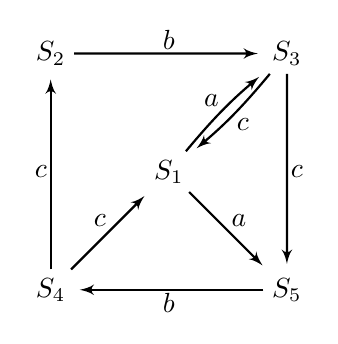
\begin{tikzpicture}[scale=1.5,%
  every node/.style={auto,inner sep=1pt},%
  every edge/.style={draw, thick,-latex',shorten >= 2pt}]
\tikzstyle{n} = [inner sep=3pt]
\node[n](s2)at(0,2){$S_2$};
\node[n](s3)at(2,2){$S_3$};
\node[n](s1)at(1,1){$S_1$};
\node[n](s5)at(0,0){$S_4$};
\node[n](s4)at(2,0){$S_5$};
\draw[->]
  (s1)edge node{$a$}(s4) edge[bend left=5pt] node{$a$}(s3)
  (s2)edge node{$b$}(s3)
  (s3)edge node{$c$}(s4) edge[bend left=5pt] node{$c$}(s1)
  (s4)edge node{$b$}(s5)
  (s5)edge node{$c$}(s2) edge node{$c$}(s1);
\end{tikzpicture}

\column{0.58\textwidth}
\begin{exampleblock}{\exercise Prove:}
\begin{enumerate}
  \item $S_1 \models \almb{a+b+c} (\evmb{b+c} \true)$\\ % after a 
  \item $S_2 \models \almb a (\evmb b \true \land \evmb c \true)$\\
  \item $S_1 \not \models \almb a(\evmb b \true \land \evmb c \true)$\\
  \item $S_2 \models \almb b \almb c(\evmb a \true \lor \evmb b \true)$\\
  \item $S_1 \models \almb b \almb c(\evmb a \true \lor \evmb b \true)$    
  \item $S_1 \not \models \almb{a+b} \evmb{b+c}(\evmb a \true)$    
%  \item $S_2 \models [a](⟨b⟩tt ∧ ⟨c⟩tt)$\\
%  \item $S_1 \not \models [a](⟨b⟩tt ∧ ⟨c⟩tt)$\\
%  \item $S_2 \models [b][c](⟨a⟩tt ∨ ⟨c⟩tt)$\\
%  \item $S_1 \models [b][c](⟨a⟩tt ∨ ⟨c⟩tt)$    
\end{enumerate}
\end{exampleblock}
\end{columns}
  
\end{slide}

%----------------------------------------------------------------------------------
% \begin{slide}{Proof system $\mathbf{K}$}\label{s:37}
% \small

% \begin{block}{Minimal modal logic}

% \begin{itemize}
% \item all formulas with the form of a \alert{propositional tautology} (including formulas which contain  modalities 
% but are truth-functionally tautologous) 
% \item all instances of  the axiom schema:
% \begin{equation*}
% \always (\phi \impp \psi) \impp (\always \phi \impp \always \psi)
% \end{equation*}
% \item two proof rules:
% \begin{align*}
% \text{if}\; \vdash \phi\; \text{and}\;  \vdash \phi \impp \psi\; \text{then}\;  \vdash \psi &\; \; \text{(\alert{modus ponens})} \\
% \text{if}\; \vdash \phi\; \text{then}\;  \vdash \always \phi &\; \; \text{(\alert{generalization})} \\
% \end{align*}
% \end{itemize}
% \end{block}
  
% \end{slide}


% %\begin{slide}{Proof system $\mathbf{K}$}
% %\begin{exampleblock}{Prove}
% %\begin{align*}
% %%  \eventual\always
% %  &\eventual(\phi \lor \psi) \to (\eventual \phi \lor \eventual \psi)
% %  \\
% %  &\eventual(\phi \lor \psi) \to \eventual \phi
% %\end{align*}
% %\end{exampleblock}
% %\end{slide}


% %----------------------------------------------------------------------------------
% \begin{slide}{Variants}\label{s:38}
% \small

% \emph{Normal modal logics} are \alert{axiomatic extensions to $\mathbf{K}$}

% \begin{itemize}
% \item
% different applications of modal logic typically validate different modal axioms;



% \item a normal modal logic is identified with the set of formulas it generates; it is said to be \alert{consistent} if it does not contain all formulas. This identification immediately induces a lattice structure on the set of all such logics.
% \end{itemize}

  
% \end{slide}

% %----------------------------------------------------------------------------------
% \begin{slide}{Variants}\label{s:39}
% \small

% Modal axioms reflect \alert{properties of accessibility relations}:
% \vspace{0.4cm}

% \begin{itemize}
% \item
% \alert{transitive} frames: $\always \phi \impp \always \always \phi$
% \item
% \alert{simple} frames: $\eventual \phi \impp \always  \phi$ 
% \item frames consisting of \alert{isolated reflexive points}: $ \phi \dimpp \always  \phi$ 
% \item frames consisting of \alert{isolated irreflexive points}: $\always  \false$ 
% \end{itemize}
% \vspace{0.3cm}

% But there are classes of frames which are not modally definable, \\
% eg, \alert{connected}, \alert{irreflexive}, \alert{containing a isolated irreflexive point} 
  
% \end{slide}



%----------------------------------------------------------------------------------
% \begin{slide}{Examples I}\label{s:15}
% \small
% \begin{block}{An automaton}
% \begin{equation*}
% %???????
% \xymatrix{
% %&&&\\
% A \; =\; \; 1 \ar[r]^{a} & 2 \ar@(ul,ur)[]^{a}  \ar[r]^{b} &3  \ar@(dl,dr)[]^{b} 
% }
% \end{equation*}
% \begin{itemize}
% \item two modalities $\evm{a}$ and $\evm{b}$ to explore the corresponding classes of transitions
% \item note that
% $$ 1 \models \evm{a} \cdots \evm{a} \evm{b} \cdots \evm{b} t$$
% where $t$ is a proposition valid only at the (terminal) state $3$. 
% \item all modal formulas of this form correspond to the strings accepted by the automaton, i.e. in language ${\cal L} = \setdef{a^mb^n}{m,n > 0}$
% \end{itemize}
% \end{block}
% \end{slide}


%----------------------------------------------------------------------------------
\begin{slide}{Other Modal Logics -- Example II}\label{s:16}
\small
\begin{block}{$(P,<)$ a strict partial order with infimum $0$}
I.e., $P=\{0, a, b, c, \ldots\}$,
\\$a\to b$ means $a<b$,
\\$a<b$ and $b<c$ implies $a<c$
\\$0 < x$, for any $x\neq 0$
\\there are no loops
\\some elements may not be comparable
\\[5mm]
% Think about TIME/progress. 0 is minimal time (smallest time)
% x 

\begin{itemize}
\item $\alert{P, x \models \always \false}\; \;$  if $x$ is a maximal element of $P$
\item $\alert{P, 0 \models \eventual \always false}\; \;$  iff  ... %$P$ contains a maximal element (> 0)
\item $\alert{P, 0 \models \always \eventual \always false}\; \;$  iff  ... %P={0} or (impossible: any larger number has a larger maximal)
\end{itemize}
\end{block}
\end{slide}





%----------------------------------------------------------------------------------
\begin{slide}{Other Modal Logics -- Example III}\label{s:18}
\small
\begin{block}{Temporal logic}
\begin{itemize}
\item $\pair{T, <}$ where $T$ is a set of time points (instants, execution states , ...) and $<$ is the \alert{earlier than} relation on $T$.
\item Thus, $\always \varphi$ (respectively, $\eventual \varphi$) means that $\varphi$ holds in all (respectively, some)  time points.
%\item \alert{origin}: Arthur Prior, an attempt to \emph{deal with temporal information from the inside, capturing the situated nature of our experience and the context-dependent way we talk about it} 
\end{itemize}
\end{block}
\end{slide}

%----------------------------------------------------------------------------------
% \begin{slide}{Examples III}\label{s:18a}
% \small

% \begin{block}{$\pair{T,<}$}
% The structure of time is a \structure{strict partial order} \\ (i.e., a transitive and asymmetric relation)
% \vspace{0.3cm}

% \noindent
% For any such structure, a new modality, $\nexts$, can be defined based on the \alert{cover} relation \alert{$\lessdot$} for $<$ 
% %(\ie, the smallest relation whose transitive closure is $<$).
% (\ie, $x\alert{\lessdot} y$ if (1) every $x<y$ and (2) there is no $z$ such that $x<z<y$).
% Thus,
% \begin{align*}
% t  \models \nexts \phi &\text{ ~~~~~~~~ \textsf{iff} ~~~} 
% \universal{t' \in \setdef{p'}{t \alert{\lessdot} t' }}{t' \models \phi} \\ &\\
% t  \models \always \phi &\text{ ~~~~~~~~ \textsf{iff} ~~~} 
% \universal{t' \in \setdef{p'}{t < t' }}{t' \models \phi} \\
% t  \models \eventual \phi &\text{ ~~~~~~~~ \textsf{iff} ~~~} 
% \existential{t' \in \setdef{p'}{t < t' }}{t' \models \phi} \\
% \end{align*}
% \end{block}

% \end{slide}

% %----------------------------------------------------------------------------------
% \begin{slide}{Examples III}\label{s:18b}
% \small

% ... but typical structures, however, are 
% % from the handybook of logics - temporal logics

% \begin{block}{Linear time structures}
% \begin{itemize}
% \item \alert{linear}: $\rcb{\forall}{x,y}{x,y \in T}{x=y ~\lor~ x<y ~\lor~ y<x}$. % NOT branching
% \item \alert{discrete}: linear and for each $t\in T$, \\
% %i) if there is a $u>t$ there is a first such $u$; ii) if there is a $u<t$ there is a last such $u$.
% $(\exists u \cdot u>t) ~\Rightarrow~ \exists u'>t$ without any $v$ s.t. $u'>v>t$ ~~~ (and its dual)
% \item \alert{dense}: if for all $t,x \in T$, if $x<t$ there is a $v\in T$ such that $x<v<t$.
% \item \alert{Dedekind complete}: if for all $S\subseteq T$ non-empty and bounded above, there is a least upper bound in $T$.
% \item \alert{continuous}: if it is both dense and Dedekind complete
% \end{itemize}
% \end{block}
% \end{slide}





%----------------------------------------------------------------------------------
\begin{slide}{Other Modal Logics -- Example IV}\label{s:19}
\small
\begin{block}{Epistemic logic (J. Hintikka, 1962)}
\begin{itemize}
\item $W$ is a set of agents 
\item $\alpha \models \alm{K_i}~\phi$ means that agent $i$ always knows that $\phi$ is true.
\item $\alpha \models \evm{K_i}~\phi$ means that agent $i$ can reach a state where he knows $\phi$.
\item $\alpha \models (\lnot \alm{K_i}~\phi) \land (\lnot \alm{K_i}~\lnot \phi)$ means that agent $i$ does not know whether $\phi$ is true or not.
% \item $\alpha \models i$ means $i$ is the current knowledge of agent $i$
% \item $\alpha \models \always j$ means the agent knows that $j$ (in the sense that at each alternative epistemic situation information $j$ is known) 
% \item $\alpha \models \eventual j$ means the agent knows that  knowledge $j$ is consistent with what the agent knows (is an epistemically acceptable alternative)
\end{itemize}
\end{block}

Many variations exist, modelling \structure{knowledge} and \structure{believes}, knowledge of \structure{who knows what}, \structure{distributed} knowledge, etc.

\end{slide}


\begin{slide}{Other Modal Logics -- Example V}\label{s:20}
\small
\begin{block}{Deontic logic (G.H. von Wright, 1951)}
\begin{itemize}
\item Obligations and permissions: \alert{must} and \structure{can} do.
\item $\alpha \models \always~\phi$ means $\phi$ is obligatory.
\item $\alpha \models \eventual~\phi$ means $\phi$ is a possibility.
% \item $\alpha \models i$ means $i$ is the current knowledge of agent $i$
% \item $\alpha \models \always j$ means the agent knows that $j$ (in the sense that at each alternative epistemic situation information $j$ is known) 
% \item $\alpha \models \eventual j$ means the agent knows that  knowledge $j$ is consistent with what the agent knows (is an epistemically acceptable alternative)
\end{itemize}
\end{block}

Each logic accepts a different set of \emph{principles} or \emph{rules} (with variations), that makes their interpretation different.

\end{slide}






%-------------------------------------------------------------------------------
% \begin{slide}{The first order connection}\label{s:20}
% \small

% \begin{block}{From modal logic}
% \vspace*{-3mm}
% \begin{equation*}
% \phi\; ::=\; \alert{p} \: \mid\: \true\: \mid\: \false\: \mid\: \neg \phi \: \mid\: \phi_1 \land \phi_2\: \mid\:
%            \phi_1 \impp  \phi_2\:   \mid\:
%            \alert{\evm{\alpha}{\phi}} \:  \mid\:
%            \alert{\alm{\alpha}{\phi}} 
% \end{equation*}
% \end{block}

% ~\\[5mm]

% \begin{block}{To first order logic}
% \vspace*{-3mm}
% \begin{equation*}
% \phi\; ::=\; \alert{P\,x} \: \mid\: \true\: \mid\: \false\: \mid\: \neg \phi \: \mid\: \phi_1 \land \phi_2\: \mid\:
%            \phi_1 \impp  \phi_2\: \mid\:
%            \alert{\rcb{\exists}{x}{}{\phi} } \: \mid\:
%            \alert{\rcb{\forall}{y}{}{\phi} }
% \end{equation*}
% \end{block}
% \end{slide}

% %------------------------------------------------------------------------------

% \begin{slide}{The first order connection}
% \small

% \only<1>{Boxes and diamonds are essentially a \alert{macro notation} to encode quantification over accessible states in a point free way. \\
% \vspace{0.2cm}}
% \begin{block}{The standard translation}

% ... to first-order logic \alert{expands} these macros:

% %\vspace{0.1cm}
% \begin{align*}
% \alert{ST_x (p)} & \alert{\,=  P\, x}\\
% ST_x (\true) & =  \true \\
% ST_x (\false) & =  \false\\
% ST_x (\neg \phi) & =  \neg ST_x (\phi)\\
% ST_x (\phi_1 \land \phi_2) & =  ST_x (\phi_1) \land  ST_x (\phi_2)\\
% ST_x (\phi_1 \impp \phi_2) & =  ST_x (\phi_1) \impp  ST_x (\phi_2)\\
% \alert{ST_x (\evm{\alpha} \phi) }& \alert{\,=  \rcb{\exists}{y}{}{(x R_m y\, \e\, ST_y(\phi))} }  \\
% \alert{ST_x (\alm{\alpha} \phi) }& \alert{\,=  \rcb{\forall}{y}{}{(x R_m y\, \impp\, ST_y(\phi))} }  \\
% \end{align*}
% \end{block}

% \only<2>{
% \centering
% \myblock{Translate: $ST_x(p \to \eventual p)$}

% }
% \end{slide}



%----------------------------------------------------------------------------------
% \begin{slide}{The first order connection}\label{s:21}
% \small

% \begin{block}{Lemma}
% For any $\phi$, $\ger{M}$ and point $w$ in $\ger{M}$, 
% \begin{equation*}
% \ger{M}, w  \models \phi \text{~~~ \textsf{iff} ~~~}  \ger{M}  \models ST_x(\phi) [x \leftarrow w]
% \end{equation*}
% \end{block}
% \begin{block}{Note}
% Note how the (unique) free variable $x$ in $ST_x$ mirrors in first-order the internal perspective: 
% \alert{assigning a value to $x$ corresponds to evaluating the modal formula at a certain state}.
% \end{block}
% \end{slide}


% %----------------------------------------------------------------------------------
% \begin{slide}{The first order connection}\label{s:22}
% \small
% The standard translation provides a \alert{bridge} between modal logic and classical logic
% which makes possible to \alert{transfer} results from one side to the other. For example,
% \vspace{0.2cm}

% \begin{block}{Compactness}
% If $\Phi$ is a set of basic modal formulas and every finite subset of $\Phi$ is satisfiable, then $\Phi$ itself is satisfiable.
% \end{block}

% \begin{block}{L\"owenheim-Skolem}
% If $\Phi$ is a set of basic modal formulas  satisfiable in at least one infinite model, then it is satisfiable in models of every infinite cardinality.
% \end{block}
% \end{slide}


% %----------------------------------------------------------------------------------
% \begin{slide}{Summing up}\label{s:23}
% \small
% \begin{itemize}
% \item Propositional modal languages are syntactically simple languages that offer a \alert{pointfree} notation for talking about \alert{relational structures}
% \item They do this from the \alert{inside}, using the modal operators to look for information at accessible states
%  \item Regarded as a tool for talking about models, any basic modal language can be seen as \alert{a fragment of first-order language}
%  \item The \alert{standard translation} systematically maps modal formulas to first-order formulas (in one free variable) and makes the quantification over accessible states explicit
% \end{itemize}
% \end{slide}



%----------------------------------------------------------------------------------
%\begin{slide}{\rdb{Exercise}}\label{s:24}
%\small
%\begin{exampleblock}{Express the following properties in Process Logic}
%\begin{itemize}
%\item \alert{inevitability of $a$}: 
%\item \alert{progress}: 
%\item \alert{deadlock or termination}: 
%\item what about
%\begin{equation*}
%\structure{\evm{-}{\false}}\; \; \; \text{and}\; \; \;  \structure{\alm{-}{\true}}\; \; \; \text{?}
%\end{equation*}
% \end{itemize}
% \end{exampleblock}
% 
%\begin{itemize}
% \item ``$-$" stands for $Act$, and ``$-x$'' abbreviates $Act-\enset{x}$
%\end{itemize}
%
%\end{slide}

%----------------------------------------------------------------------------------
\begin{slide}{Exercise}\label{s:25}
\small

\begin{columns}[T]

\col[0.70]{
  \doExercise{Express the properties in Process Logic}{
  \exerciseBack
    ~\\[-5mm]
  \begin{itemize}
  \item \alert{inevitability of $a$}: \only<2->{\structure{$\evm{-}{\true} \land \alm{-a}{\false}$}}
  \item \alert{progress (can act)}: %\only<3->{\structure{$\evm{-}{\true}$}}
  \item \alert{deadlock or termination (is stuck)}: %\only<4->{\structure{$\alm{-}{\false}$}}
  % \visible<4->{\item what about
  % \begin{equation*}
  % \structure{\evm{-}{\false}}\; \; \; \text{and}\; \; \;  \structure{\alm{-}{\true}}\; \; \; \text{?}
  % \end{equation*}}
  \end{itemize}
  }

  \exerciseAdd
  \doExercise{What does this mean?}{
  \exerciseBack
  \exerciseBack
    ~\\[-5mm]
    \begin{enumerate}
      \item ${\evm{-}{\false}}$
      \item ${\alm{-}{\true}}$
    \end{enumerate}
  }

  ``$-$" stands for $\sum_{a\in Act}a$, and ``$-x$'' abbreviates $\sum_{a\notin Act}a$
}
\col[0.28]{
    \begin{block}{Recall syntax}
  \begin{align*}
  \phi ~::&=~ \true
          \\&~\,\mid~ \false
          \\&~\,\mid~ \neg \phi 
          \\&~\,\mid~ \phi_1 \land \phi_2
          \\&~\,\mid~ \phi_1 \impp  \phi_2  
          \\&~\,\mid~ \evm{\structure{K}}{\phi}  
          \\&~\,\mid~ \alm{\structure{K}}{\phi} 
  \end{align*}
  ~\\
  where $\structure{K := a ~|~ K+K}$
  \end{block}
}
\end{columns}
\end{slide}
\exerciseAdd
\exerciseAdd


\begin{slide}{Express the following using Process Logic}
  \doExercise{Coffee-machine}{
    \\[-5mm]
    \begin{enumerate}
      \item The user can have \alert{tea} or \alert{coffee}.
      \item The user can have \alert{tea} but not \alert{coffee}.
      \item The user can have \alert{tea} after having 2 consecutive \alert{coffees}.
    \end{enumerate}
  }

  \doExercise{$a$'s and $b$'s}{
    \\[-5mm]
    \begin{enumerate}
      \item It is possible to do \alert{$a$} after 3 \alert{$b$}'s, but not more than 1 \alert{$a$}.
      \item It must be possible to do \alert{$a$} after [doing \alert{$a$} and then \alert{$b$}].
      \item After doing \alert{$a$} and then \alert{$b$}, it is not possible to do \alert{$a$}.
    \end{enumerate}
  }

\end{slide}



%----------------------------------------------------------------------------------
\begin{slide}{Express the following using Process Logic}\label{s:26}
\small
\doExercise{Taxi network}{
\\[-4mm]
\begin{itemize}
\item $\phi_0 =$ \emph{In a taxi network, a car can \alert{col}{lect} a passenger or be \alert{allo}{cated} by the Central to a pending service}
\item $\phi_1 =$ \emph{This applies only to cars already \alert{on-service}}
\item $\phi_2 =$
 \emph{If a car is \alert{allo}{cated} to a service, it must first \alert{col}{lect} the passenger and then \alert{plan} the route}
\item $\phi_3 =$ \emph{On detecting an \alert{emergency} the taxi becomes inactive}
\item $\phi_4 =$ \emph{A car \alert{on-service} is not inactive}
\end{itemize}
}
\end{slide}


%----------------------------------------------------------------------------------
% \begin{slide}{Exercise}\label{s:27}
% \small
% \doExercise{Process logic: The taxi network example}{
% \begin{itemize}
% \item $\phi_0 =\; \evm{rec,alo}{\true}$ 
% \item $\phi_1 =\;  \alm{onservice}{\evm{rec,alo}{\true}}\; $ or\\
% $\phi_1 =\;   \alm{onservice}{\phi_0}$
% \item $\phi_2 =\;  \alm{alo}{\evm{rec}{\evm{plan}{\true}}}$
% \item $\phi_3 =\;  \alm{sos}{\alm{-}{\false}}$
% \item $\phi_4 =\;  \alm{onservice}{\evm{-}{\true}}$
% \end{itemize}
% }
% \end{slide}


%----------------------------------------------------------------------------------
% \begin{slide}{Exercise}\label{s:28}
% \small
% \begin{exampleblock}{Standard translation to FOL}
% \begin{itemize}
% \item Explain how propositional symbols and modalities are translated to first-order logic?
% \item In what sense can modal logic be regarded as a \alert{pointfree} version of a FOL fragment?
% \item Compute  $ST_x (p \imp \evm{\alpha}{p})$ 
% % ST_x p  --> ST_x \evm{\alpha}{p}
% % = P x  --> exists y : y R_m x  &  P y
% \end{itemize}
% \end{exampleblock}
% \end{slide}



\begin{slide}{Process Logic + regular expressions}
  

  \begin{block}{Process Logic with regular expressions}
  \begin{equation*}
  \phi\; ::=\; \true\: \mid\: \false\: \mid\: \neg \phi \: \mid\: \phi_1 \land \phi_2\: \mid\:
             \phi_1 \impp  \phi_2\:   \mid\:
             \evm{\alert{\alpha}}{\phi} \:  \mid\:
             \alm{\alert{\alpha}}{\phi} 
  \end{equation*}
  % where $\alert{E}$ is a \alert{regular expression over $Act$}
  where $\alpha\in ACT$ are structured actions over a set $Act$:
  \begin{align*}
    \alert{\alpha := a\in Act~~|~~\alpha;\alpha~~|~~\alpha+\alpha~~|~~\alpha^{*}}
  \end{align*}
  \vspace*{-4mm}
  \end{block}

  % \begin{block}{Process Logic Syntax}
  % \begin{equation*}
  % \phi\; ::=\; \true\: \mid\: \false\: \mid\: \neg \phi \: \mid\: \phi_1 \land \phi_2\: \mid\:
  %            \phi_1 \impp  \phi_2\:   \mid\:
  %            \evm{\alert{E}}{\phi} \:  \mid\:
  %            \alm{\alert{E}}{\phi} 
  % \end{equation*}
  % where $\alert{E}$ is a \alert{regular expression over $Act$}
  % \end{block}

  \only<1>{
  More expressive than Process Logic. Used by mCRL2.}

  \only<2>{~\\[-11mm]
  \begin{exampleblock}{Examples}
  \begin{itemize}
    \item ``$\evm{a;b;c}{\true}$'' means ``$\diam{a}\diam{b}\diam{c}\,\true$'' 
    \item ``$\alm{a;b;c}{\false}$'' means ``$\boxx{a}\boxx{b}\boxx{c}\,\false$'' 
    \item ``$\evm{a^{*};b}{\true}$'' means that $b$ can be taken after some number of $a$'s. 
    \item ``$\evm{-^{*};a}{\true}$'' means that $a$ can \alert{eventually} be taken
    \item ``$\boxx{-^{*}}\evm{a+b}{\true}$'' means it is \alert{always}  possible to do $a$ or $b$
  \end{itemize}
  \end{exampleblock}
  }

\end{slide}



\begin{slide}{Exercises} %: Properties of our coffee machine}
  ~\\[-6mm]
  \splittwo{0.35}{0.65}{
    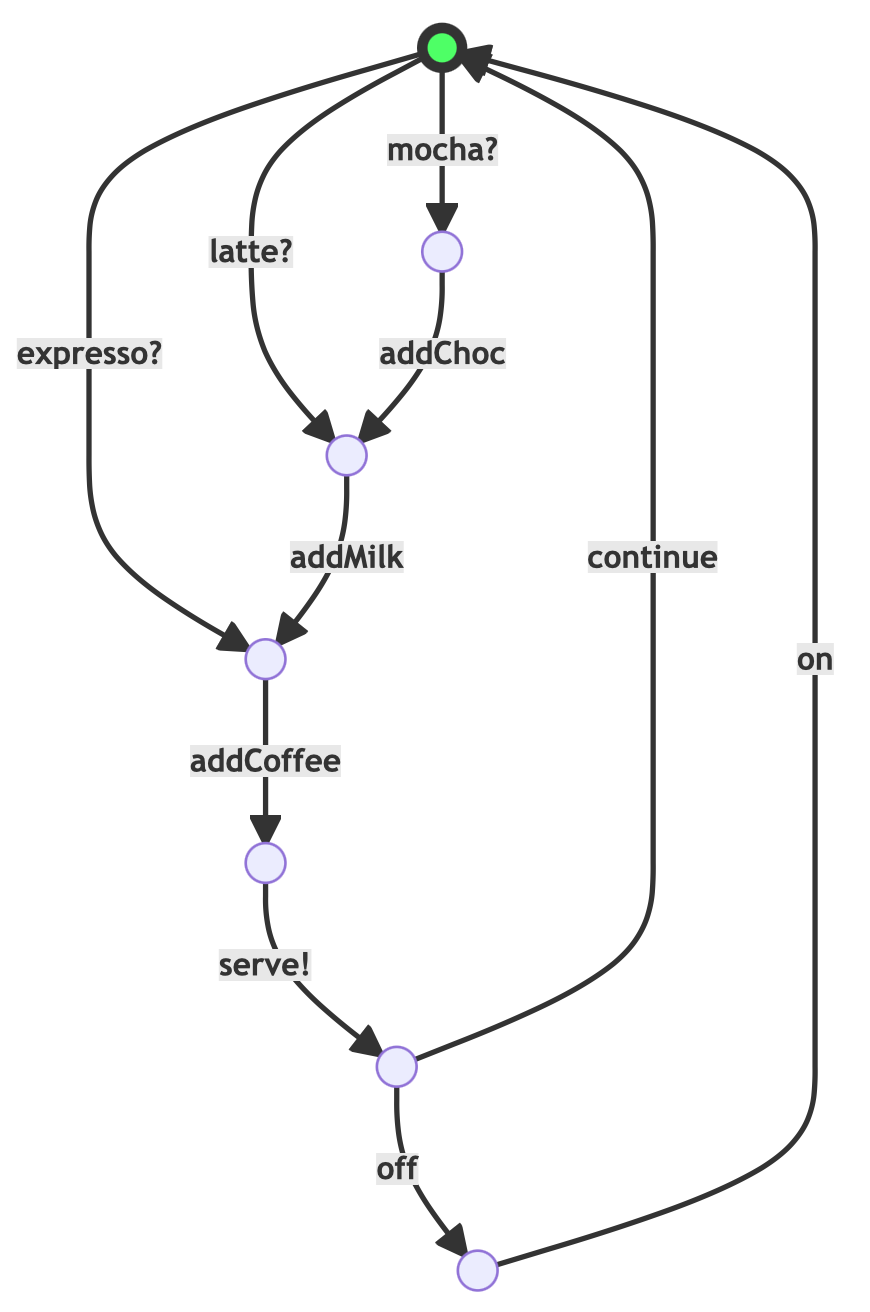
\includegraphics[width=\textwidth]{images/coffee-model.png}
  }{
    \doExercise{What does this mean?}{
    \vspace*{-8mm}
    \begin{itemize}
      \item $\evmb{-^{*};serve!} \true$
      \item $\almb{-^{*};(addChoc+addMilk);serve!} \false$
      \item $\almb{-^{*};addCoffee}\evmb{serve!} \true$
      \\~
      \item $\evmb{-}\true$
      \item $\almb{-^{*}}\evmb{-}\true$
      \item $\almb{-^{*};a}\evmb{b}\true$
      \item $\almb{-^{*};send} \evmb{(-send)^{*};recv}\true$
    \end{itemize}
    }
  }
\end{slide}


\begin{slide}{Exercises} %: Properties of our coffee machine}
  ~\\[-6mm]
  \splittwo{0.35}{0.65}{
    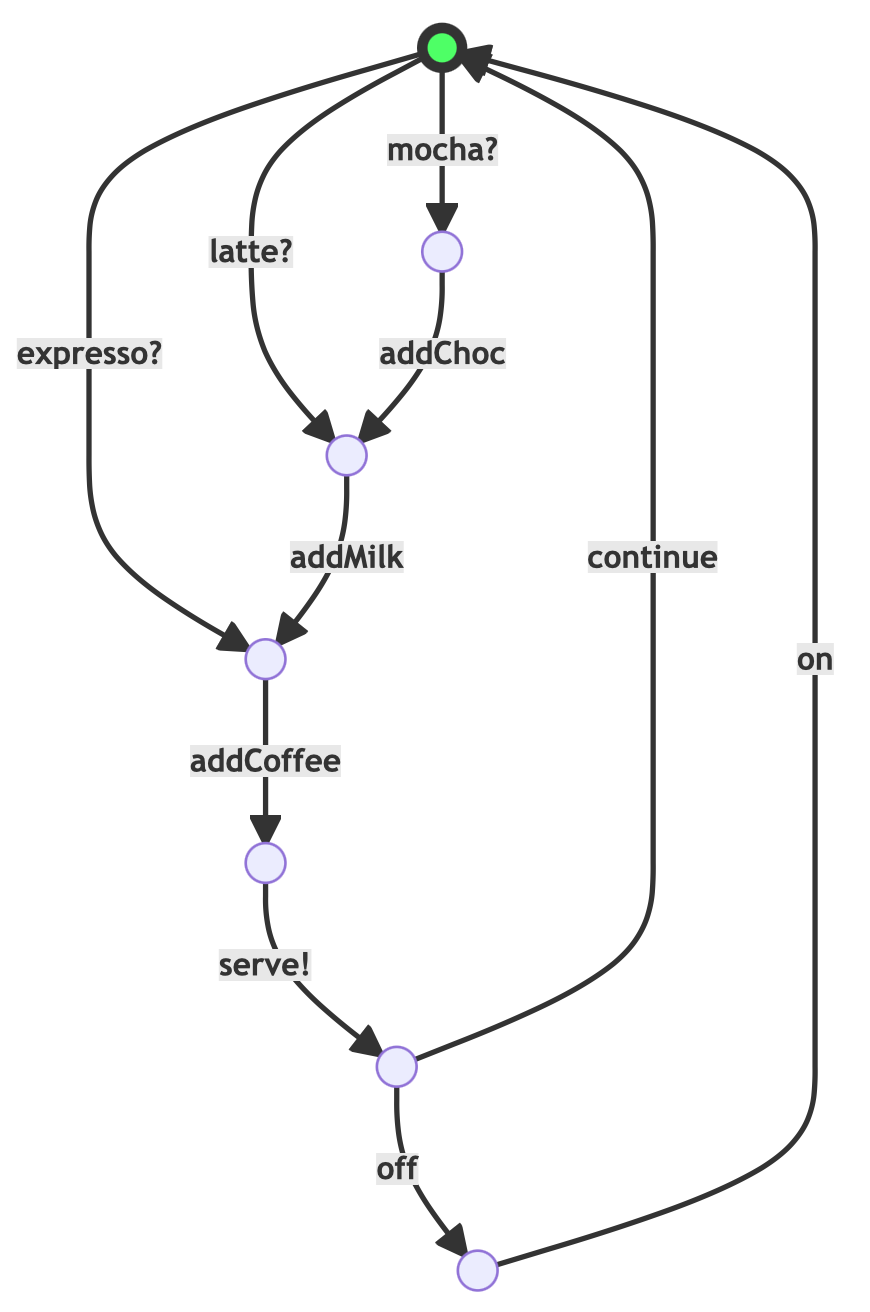
\includegraphics[width=\textwidth]{images/coffee-model.png}
  }{
    \doExercise{Express using logic}{
    \vspace*{-8mm}
    \begin{enumerate}
      \item The user \structure{can only have} \alert{coffee} after the \alert{coffee button} is pressed.
      \item The used \structure{must have} \alert{coffee} after the \alert{coffee button} is pressed.
      \item It is always possible to \alert{turn off} the coffee machine.
      \item It is always possible to reach a state where the coffee machine can be \alert{turned off}.
      \item It is never possible to \alert{add chocolate} right after pressing the \emph{latte button}.
    \end{enumerate}
    }
  }
\end{slide}


% \begin{slide}{Exercises}
% \small

% \begin{columns}[T]
% \col[0.34]{\doExercise{What does this mean?}{
%   \vspace*{-8mm}
%   \begin{enumerate}
%     \item $\evm{-}\true$
%     \item $\boxx{-^{*}}\evm{-}\true$
%     \item $\boxx{-^{*}.a}\evm{b}\true$
%     \item $\boxx{-^{*}.send}$\\$\evm{(-send)^{*}.recv}\true$
%   \end{enumerate}
% }}

% \col[0.65]{\doExercise{Express using logic}{
%   \vspace*{-8mm}
%   \begin{enumerate}
%     \item The user \structure{can only have} \alert{coffee} after the \alert{coffee button} is pressed.
%     \item The used \structure{must have} \alert{coffee} after the \alert{coffee button} is pressed.
%     \item It is always possible to \alert{turn off} the coffee machine.
%     \item It is always possible to reach a state where the coffee machine can be \alert{turned off}.
%     \item It is never possible to \alert{add chocolate} right after pressing the \emph{latte button}.
%   \end{enumerate}
% }}
% \end{columns}
  
% \end{slide}


\begin{frame}
  \huge\centering
  mCRL2 Tools
  \\[5mm]\large
  Slides 3:\\\url{https://fm-dcc.github.io/sv2425/slides/3-mcrl2.pdf}
\end{frame}



\section{Bisimulation and modal equivalence}
%----------------------------------------------------------------------------------
\begin{slide}{Bisimulation (of models)}\label{s:29}
\begin{block}{Definition}
Given two models $\ger{M} = \pair{\ger{L}, V}$ and $\ger{M}' = \pair{\ger{L}', V'}$, a \structure{bisimulation 
of $\ger{L}$ and $\ger{L}'$} is also a \alert{bisimulation of $\ger{M}$ and $\ger{M}'$} if,
\\
\begin{center}
  whenever $s~R~s'$, then $V(s)= V'(s')$
\end{center}

%  $\subseteq W \times W'$  st whenever $w S w'$ one has that
% \begin{enumerate}
% \item points $w$ and $w'$ satisfy the same propositional symbols
% \item if $w R v$, then there is a point $v'$ in $\ger{M}'$ st  $w' R' v'$ and $v S v'$ \hspace{0.3cm} (\alert{zig})
% \item if $w' R' v'$, then there is a point $v$ in $\ger{M}$ st  $w R v$ and $v S v'$ \hspace{0.3cm} (\alert{zag})
% \end{enumerate}
\end{block}
%\begin{block}{Note}
%Note the relation to the notion of bisimulation in transition systems, independently discovered by Park (1982) in Computer Science.
%\end{block}
\end{slide}

%----------------------------------------------------------------------------------
%\begin{slide}{Bisimulation (of models)}\label{s:30}
%\small
%\begin{block}{Definition}
%\begin{itemize}
%\item Bisimulations can be used to \alert{expand} or \alert{contract} models (cf via  tree unraveling and contraction)
%\item Bisimulation vs model constructions (\alert{disjoint union}, \alert{generated submodels} and \alert{bounded morphisms})
%\end{itemize}
%\end{block}
%\begin{block}{Note}
%Note the relation to the notion of bisimulation in transition systems, independently discovered by Park (1982) in Computer Science.
%\end{block}
%\end{slide}



%----------------------------------------------------------------------------------
\begin{slide}{Invariance and definability}\label{s:31}
\small
\begin{block}{Lemma (invariance: bisimulation implies modal equivalence)}
Given \structure{two models} $\ger{M}$ and $\ger{M}'$, and a \alert{bisimulation} 
$R$ between their states:
\\[5mm]
~~\alert{if} two states $s, s'$ are related by $R$ (i.e. $s R s'$),\\
~~\alert{then} $s, s'$  satisfy the same basic modal formulas.\\
~~~~~~~~~\textcolor{black!50}{(i.e., for all $\phi$:
  ~~~$\ger{M},s \models \phi ~\Leftrightarrow~ \ger{M}',s' \models \phi$)}
% or: M,x |= φ iff N,y |= φ for all modal formulas φ
 \end{block}


\begin{alertblock}{Hence}
  \centering
  Given 2 models $\ger{M}$ and $\ger{M'}$, if you can find $\phi$ such that
  \\[4mm]
  $\ger{M}\models \phi$ and $\ger{M'}\not \models \phi$
  \\[4mm]
  (or vice-versa) then they are NOT bisimilar.
  
\end{alertblock}

% \begin{block}{Applications}
% \begin{itemize}
% \item to prove bisimulation failures
% \item to show the undefinability of some structural notions, e.g. \alert{irreflexivity is modally undefinable}
% \item  to show that typical model constructions are satisfaction preserving
% \item ...
% \end{itemize}
% \end{block}
\end{slide}


% %-------------------------------------------------------------------------------
% \begin{frame}{Exercise}
% \begin{exampleblock}{Find characterising formulas}
% \centering
% \wrap[b]{
% \begin{tikzpicture}
%   \node(1)at(0,0){1};   \node(2)at(1,1){2};
%   \node(3)at(1,-1){3};  \node(4)at(2,0){4};
%   \draw[->] (1)edge(2)edge(3)edge(4) (2)edge(4)edge[loop above]() (3)edge(4);
% \end{tikzpicture}}
% ~~~~~~~~~~~
% \wrap[b]{\begin{tikzpicture}
%   \node(1)at(0,0){5};   \node(2)at(1,1){6};
%   \node(3)at(1,-1){7};  \node(4)at(2,0){8};
%   \draw[->] (1)edge(2)edge(3)edge(4) (2)edge(4) (3)edge(4);
% \end{tikzpicture}}
% \\[4mm]
% \eg, (4) is the only world satisfying $\Box\bot$
% \end{exampleblock}
% %%%
% % from ML for open minds
% % 3: <>[]ff /\ [][]ff --- (also [][]ff?)
% % 1: <>(3:)
% % 2: <><>tt /\ not(1:)
% % tip: last point as negation of all others...
% % on the rhs: 2 becomes 3.
% \end{frame}

% %----------------------------------------------------------------------------------
% \begin{slide}{Frame definability}\label{s:32}
% \small
% \begin{itemize}
%   \item A modal formula is valid on a frame if it is true under \red{every valuation} at \red{every world} (i.e., it cannot be refuted)
%   \item The class of frames defined by a modal formula $\phi$ are those where $\phi$ is valid.
%   \item Example: $\eventual\eventual p \to \eventual p$ defines transitivity:\\
%   ~~~~$\ger{F}=\pair{W,R}$ is transitive iff \red{for all $V$ and $w$},\\
%   ~~~~$\pair{\ger{F},V},w\models \eventual\eventual p \to \eventual p $
% \end{itemize}
% \end{slide}
% %----------------------------------------------------------------------------------
% \begin{slide}{Exercise}\label{s:32}
% \small

% \begin{exampleblock}{Exercise: other properties}
% \begin{enumerate}
%   \item Transitivity: \structure{$\eventual\eventual p \to \eventual p$}
%   \item Reflexivity: \visible<2->{\structure{$p \to \eventual p$}}
%   \item Symmetry:    \visible<2->{\structure{$p \to \always \eventual p$}}
%   \item Confluence:  \visible<2->{\structure{$\eventual\always p \to \always \eventual p$}}
%   \item Irreflexibility:  \visible<2->{\alert{Not possible}}
% \end{enumerate}
% \end{exampleblock}

% \end{slide}

%----------------------------------------------------------------------------------

\begin{slide}{Exercise}\label{s:32}
\small
\doExercise{Bisimilarity and modal equivalence}{
Consider the following transition systems:
\begin{equation*}
%??????
\xymatrix{
%&&&\\
&&& 5 &\\
1 \ar@(ul,ur)[]  \ar[r] & 2 & \hspace{0.3cm} & 3 \ar[u] \ar[d]  \ar@/^/[r]   & 4 \ar@/^/[l]  \\
&&& 6 &
}
\end{equation*}
Give a modal formula that can be satisfied at point $1$ but not at $3$.
%[]([]false \/ <>[]false) - after any step it either deadlocks in one or 2 steps.
% book - Modalities and Multimodalities
% It is enough to see that (lhs) and (another irreflexive model) are bisimilar, although one is reflexive and the other not.
% IF irreflexivity were modally definable, the modal formula PSI which defines it would have to be invariant under bisimulations.
% BUT if PSI were to be true in (v-another-irr-model) then it would be true in (lhs) by the invariance lemma, which is impossible since (u-lhs) is a reflexive point.
% \item Show that  \alert{irreflexivity} is modally undefinable.
% \\(\ie, no formula that characterises a irreflexive system)
% \item Prove the invariance lemma.
}
\end{slide}


\begin{slide}{Exercise}
  \begin{exampleblock}{\exercise Find distinguishing modal formula}
    \begin{align*}
    1)~~~&&&
    \wrap{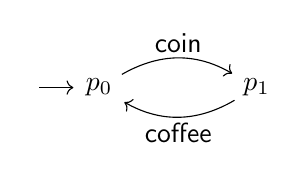
\begin{tikzpicture}[aut]
      \node[sst,initial left,final]  (s_0) {$p_0$};
      \node[sst] (s_1) [right of=s_0] {$p_1$};
      \path[->]
        (s_0) edge[bend left] node {coin} (s_1)
        (s_1) edge[bend left] node {coffee} (s_0);
    \end{tikzpicture}}
    &&
    \wrap{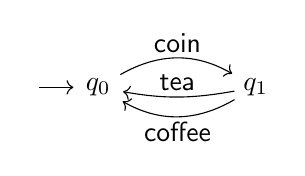
\begin{tikzpicture}[aut]
      \node[sst,initial left,final]  (s_0) {$q_0$};
      \node[sst] (s_1) [right of=s_0] {$q_1$};
      \path[->]
        (s_0) edge[bend left] node {coin} (s_1)
        (s_1) edge[bend left] node {coffee} (s_0)
        (s_1) edge[bend left=10] node[above] {tea} (s_0);
    \end{tikzpicture}}
    \\[3mm]
    2)~~~&&&
    \wrap{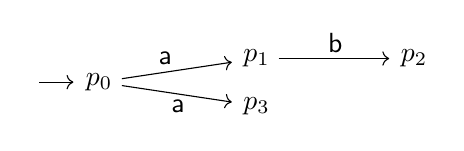
\begin{tikzpicture}[aut]
      \node[sst,initial left,final]  (s_0) {$p_0$};
      \node[sst] (s_1) [right of=s_0, yshift=3mm] {$p_1$};
      \node[sst] (s_2) [right of=s_1] {$p_2$};
      \node[sst] (s_3) [right of=s_0, yshift=-3mm] {$p_3$};
      \path[->]
        (s_0) edge  node {a} (s_1) edge node[below]{a} (s_3)
        (s_1) edge  node {b}  (s_2);
    \end{tikzpicture}}
    &&
    \wrap{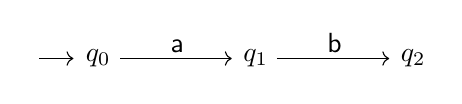
\begin{tikzpicture}[aut]
      \node[sst,initial left,final]  (s_0) {$q_0$};
      \node[sst] (s_1) [right of=s_0] {$q_1$};
      \node[sst] (s_2) [right of=s_1] {$q_2$};
      \path[->]
        (s_0) edge  node {a} (s_1)
        (s_1) edge  node {b}  (s_2);
    \end{tikzpicture}}
    \\[3mm]
    3)~~~&&&
    \wrap{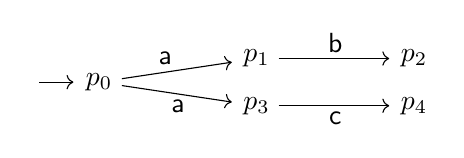
\begin{tikzpicture}[aut]
      \node[sst,initial left,final]  (s_0) {$p_0$};
      \node[sst] (s_1) [right of=s_0, yshift=3mm] {$p_1$};
      \node[sst] (s_2) [right of=s_1] {$p_2$};
      \node[sst] (s_3) [right of=s_0, yshift=-3mm] {$p_3$};
      \node[sst] (s_4) [right of=s_3] {$p_4$};
      \path[->]
        (s_0) edge  node {a} (s_1) edge node[below]{a} (s_3)
        (s_1) edge  node {b}  (s_2)
        (s_3) edge  node[below] {c}  (s_4);
    \end{tikzpicture}}
    &&
    \wrap{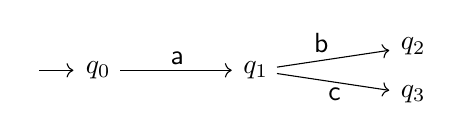
\begin{tikzpicture}[aut]
      \node[sst,initial left,final]  (s_0) {$q_0$};
      \node[sst] (s_1) [right of=s_0] {$q_1$};
      \node[sst] (s_2) [right of=s_1, yshift=3mm] {$q_2$};
      \node[sst] (s_3) [right of=s_1, yshift=-3mm] {$q_3$};
      \path[->]
        (s_0) edge  node {a} (s_1)
        (s_1) edge  node {b}  (s_2)
        (s_1) edge node[below]{c} (s_3);
    \end{tikzpicture}}
    \end{align*}
\end{exampleblock}

\end{slide}
%----------------------------------------------------------------------------------
% \begin{slide}{Invariance and definability}\label{s:33}
% \small
% To prove the converse of the invariance lemma requires passing to an \alert{infinitary} modal language  with arbitrary (countable) conjunctions and disjunctions. Alternatively, and more usefully, it can be shown  for \alert{finite} models:
% \begin{block}{Lemma (modal equivalence implies bisimulation)}
% \red{If} two points $w, w'$ from two finite models $\ger{M} = \pair{\pair{W, R}, V}$ and $\ger{M}' = \pair{\pair{W', R'}, V'}$ satisfy the same modal formulas,
% \\
% \red{then} there is a bisimulation $S \subseteq W \times W'$  such that $w S w'$.
%  \end{block}
% \end{slide}

% %----------------------------------------------------------------------------------
% \begin{slide}{Invariance and definability}\label{s:34}
% \small
% \begin{block}{Note}
% \begin{itemize}
% \item The result can be \structure{weakened} to \alert{image-finite} models.
% \item Combining this result with the invariance lemma one gets the so-called \structure{modal equivalence theorem} stating that, for image-finite models, bisimilarity and modal equivalence coincide. The result is also known as the \structure{Hennessy-Milner theorem} who first proved it for process logics.
% %\item the situation is similar to what happens in first-order logic: first-order formulas are invariant for \alert{potential isomorphism}, but the converse only holds in a weak formulation: two models are potentially isomorphic iff they have the same complete theory in the \alert{infinitary} first-order logic.
% \end{itemize}
% \end{block}

% \begin{exampleblock}{Exercise}
% \begin{itemize}
% \item Give an example of modally equivalent states in different Kripke structures which fail to be bisimilar.
% % infinite models: one modal formula satisfies 2 non-bisimilar (infinite) models
% % m1: infinte branching of finite steps 0, 0-1, 0-1-2, 0-1-2-3,...
% % m2: same as m1, but with an extra infinitly long branch
% % For every point, 
% % https://books.google.pt/books?id=ql_dBtNOOeAC&pg=PA63&lpg=PA63&dq=not+bisimilar+infinite&source=bl&ots=ONMAmSjJ2E&sig=XpHSBzXyjJ0TUmImDu1Eg8MFnd4&hl=en&sa=X&redir_esc=y#v=onepage&q=not%20bisimilar%20infinite&f=false
% \end{itemize}
% \end{exampleblock}
% \end{slide}


% %----------------------------------------------------------------------------------
% \begin{slide}{Invariance and definability}\label{s:35}
% \small

% \begin{block}{Lemma (modal logic vs first-order)}
% The following are equivalent for all first-order formulas $\phi(x)$ in one free variable $x$:
% \begin{enumerate}
% \item $\phi(x)$ is invariant for bisimulation.
% \item $\phi(x)$ is equivalent to the standard translation of a basic modal formula.
%  \end{enumerate}
%   \end{block}
  
%  Therefore:\\
%  \alert{the basic modal language corresponds to the fragment of their first-order correspondence language that is invariant for bisimulation}
% \end{slide}


% %----------------------------------------------------------------------------------
% \begin{slide}{Invariance and definability}\label{s:36}
% \small

% \begin{itemize}
% \item the basic modal language (interpreted over the class of all models) is computationally better behaved than the corresponding first-order language (interpreted over the same models)
% \item ... but clearly less  expressive 
% \end{itemize}

% \begin{center}
% \begin{tabular}{|c|c|c|c|}
% \hline
%  & model checking & satisfiability \\ \hline
%  ML & PTIME & PSPACE-complete  \\
%  FOL & PSPACE-complete & undecidable \\
%  \hline
% \end{tabular}
% \end{center}

  
%   \vspace{0.2cm}
%  \alert{What are the trade-offs? Can this better computational behaviour be lifted to more expressive modal logics? }
% \end{slide}


%-------------------------------------------------------------------------------
% \begin{slide}{mCRL2 - modal logic}
% \newcommand{\expr}{\mathit{mod}}
% \newcommand{\midd}{\,~|~\,}
% \centering
% \begin{block}{Syntax (simplified)}
% \begin{align*}
%   \phi =&~ \mcode{true} \midd \mcode{false} \midd
%           \mcode{forall x:T.}\phi \midd \mcode{exists x.:T}\phi \\|&~
%           \phi~OP~\phi \midd \mcode{!}\phi \midd
%           \mcode{[$\structure{\expr}$]}\phi \midd \mcode{<$\structure{\expr}$>}\phi \midd \ldots
% \\[3mm]
% \structure{\expr} =&~ \structure{\alpha} \midd \mcode{nil} \midd \expr\mcode{+}\expr \midd
%         \expr\mcode{.}\expr \midd \expr\mcode{*} \midd \expr\mcode{+}
% \\[1mm]
% \structure{\alpha} =&~ \mcode{a(d)} \midd \mcode{a|b|c} \midd
%           \mcode{true} \midd \mcode{false} 
%           \midd
%           \alpha~OP~\alpha \midd \mcode{!}\alpha
%           \\|&~
%           \mcode{forall x:T.}\alpha \midd \mcode{exists x:T.}\alpha 
%           \midd
%           \ldots
% \end{align*}
% \end{block}
% %~\\[2mm]
% where $OP = \set{\mcode{&&},\mcode{||},\mcode{=>}}$ ~~and~~
% $T = \set{Bool, Nat, Int, \ldots}$

% \begin{exampleblock}{Example}
% ``\code{[true*.a]<b>true}'' means \emph{``whenever an \code{a} appears after any number of steps, it must be immediately followed by \code{b}''}. 
% \end{exampleblock}
% \end{slide}

% %-------------------------------------------------------------------------------
% \begin{slide}{mCRL2 toolset overview}
%   \centering
  
%   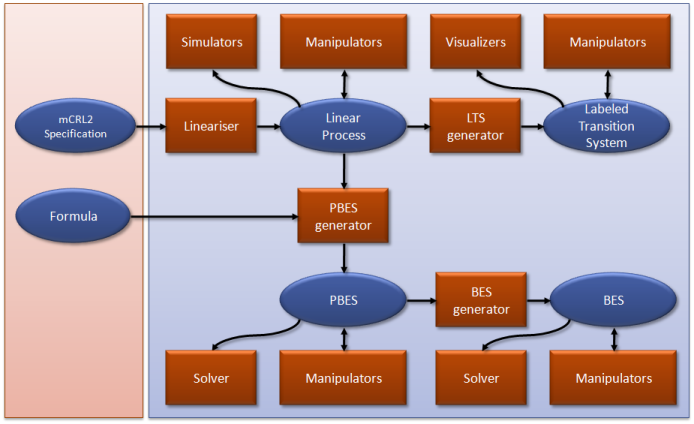
\includegraphics[width=\textwidth]{images/mcrl2-toolset.png}

%   -- mCRL2 tutorial: Verification part --
% \end{slide}



 \section{Richer modal logics}


%----------------------------------------------------------------------------------
\begin{slide}{Richer modal logics}\label{s:40}
\small

can be obtained in different ways, e.g.

\begin{itemize}
\item axiomatic extensions
\item introducing more complex satisfaction relations
\item \alert{support novel semantic capabilities}
\item ...
\end{itemize}
 
 Examples
 \begin{itemize}
 \item richer temporal logics
\item hybrid logic
 \item modal $\mu$-calculus 
\end{itemize}
\end{slide}


%----------------------------------------------------------------------------------
%\begin{slide}{Temporal logics with $\mathcal{U}$ and $\mathcal{S}$}\label{s:41}
%\small
%\begin{block}{Until and Since}
%\begin{align*}
%\ger{M}, w  &\models \phi\, \mathcal{U}\, \psi & \text{ ~~ \textsf{iff} ~~} &
%\text{there exists}\; v \in W \;\text{st}\; w R v\; \text{and}\; \ger{M}, v \models \psi,\\
%& & & \text{and for all}\; u\; \text{st}\; w R u\; \text{and}\; u R v,\; \text{one has}\;  \ger{M}, u \models \phi\\
%\ger{M}, w  &\models \phi\, \mathcal{S}\, \psi & \text{ ~~ \textsf{iff} ~~} &
%\text{there exists}\; v \in W \;\text{st}\; v R w\; \text{and}\; \ger{M}, v \models \psi,\\
%& & & \text{and for all}\; u\; \text{st}\; v R u\; \text{and}\; u R w,\; \text{one has}\;  \ger{M}, u \models \phi
%\end{align*}
%\end{block}
%%
%\begin{itemize}
%\item note the $\exists\, \forall$ qualification pattern: these operators are neither diamonds nor boxes.
%\item  more expressive --- e.g. helpful to express \alert{guarantee} properties, 
%e.g. \structure{some event will happen, and a certain condition will hold until then}
%\end{itemize}
%\end{slide}
%
%----------------------------------------------------------------------------------
\newcommand{\Until}{\mathop{\mathcal{U}}} 
\newcommand{\Since}{\mathop{\mathcal{S}}} 
\begin{frame}{Temporal Logics with $\Until$ and $\Since$}
\begin{block}{Until and Since}
  \begin{align*}
    \ger{M},s & \models \phi\Until\psi
      & \text{iff}~~& \text{there \structure{exists} $r$ st
                      $s\alert{\leq}r$ and $\ger{M},r \models \psi$, and} \\
      && & \text{\structure{for all} $t$ st $s \alert{\leq} t \alert{<} r$,
                 one has $\ger{M},t \models \phi$}
    \\[2mm]
    \ger{M},s & \models \phi\Since\psi
      & \text{iff}~~& \text{there \structure{exists} $r$ st
                      $r\alert{\leq}s$ and $\ger{M},r \models \psi$, and} \\
      && & \text{\structure{for all} $t$ st $r \alert{<} t \alert{\leq} s$,
                 one has $\ger{M},t \models \phi$}
  \end{align*}
\end{block}
%
\begin{itemize}
\item Defined for temporal frames $\pair{T,<}$ (transitive, asymmetric).
\item note the $\exists\, \forall$ qualification pattern: these operators are neither diamonds nor boxes.
\item  More general definition for other frames -- it becomes more expressive than modal logics.
\end{itemize}
\end{frame}

%----------------------------------------------------------------------------------
\begin{frame}{Exercise}
\begin{exampleblock}{Temporal logics - rewrite using $\Until$}
\begin{itemize}
  \item $\eventual \psi = \only<2->{\blue{tt \Until \psi}}$
  \item $\always \psi = \only<3>{\blue{\lnot(\eventual \lnot \psi)} = \blue{
                        \lnot(tt \Until \lnot\psi)}}$
\end{itemize}
\end{exampleblock}
  
\end{frame}


%\begin{slide}{Exercise}\label{s:42}
%\small
%\begin{exampleblock}{Temporal logics}
%\begin{itemize}
%\item Show that  $\mathcal{U}$ is modally undefinable.\\
%\emph{Hint} Consider the following transition structures and formula $\false\, \mathcal{U}\, \true$:
%
%\begin{equation*}
%%????????
%\xymatrix{
%%&&&\\
%1 \ar@(ul,ur)[]   & \hspace{0.3cm} & 2  \ar@/^/[r]   & 3 \ar@/^/[l]  
%}
%\end{equation*}
%\item Would this be the case if we restrict ourselves to transitive, irreflexive models?
%\end{itemize}
%\end{exampleblock}
%\end{slide}


%----------------------------------------------------------------------------------
\begin{slide}{Linear temporal logic (LTL)}\label{s:44}
\small

\[
\phi\, := \; \true \mid p \mid  \phi_1 \wedge \phi_2 \mid \neg \phi \mid \blue\nexts \phi \mid  \phi_1 \,\blue\Until\, \phi_2 %\mid \eventual \phi \mid \always \phi
\]
\vspace{0.5cm}
\begin{center}
\begin{tabular}{|l|c|}
\hline
mutual exclusion  & $\blue\always (\neg c_1 \vee \neg c_2)$ \\
 liveness & $\blue\always \blue\eventual c_1 \wedge \blue\always \blue\eventual c_2$\\
starvation freedom  & $(\blue\always \blue\eventual w_1 \impp \blue\always \blue\eventual c_1) \wedge
(\blue\always \blue\eventual w_1 \impp \blue\always \blue\eventual c_1)$ \\
progress & $\blue\always (w_1 \impp \blue\eventual c_1)$\\
weak fairness & $\blue\eventual \blue\always w_1 \, \impp \blue\always \blue\eventual c_1$\\
eventually forever & $\blue\eventual \blue\always w_1$\\
\hline
\end{tabular}  
\end{center}

\begin{itemize}
\item First temporal logic to reason about reactive systems [Pnueli, 1977]
\item Formulas are interpreted over \structure{execution paths}
\item Express \structure{linear-time properties}
\end{itemize}
\end{slide}

%----------------------------------------------------------------------------------
\begin{slide}{Computational tree logic (CTL, CTL*)}\label{s:45}
\small

 \alert{state} formulas to express  properties of a state:
\[
\Phi\, := \; \true \mid \Phi \wedge \Phi \mid \neg \Phi \mid \alert{\exists} \psi \mid \alert{\forall} \psi
\]


\structure{path} formulas to express properties of a path:
\[
\psi\, := \; \structure{\nexts} \Phi \mid  \Phi \structure{\until} \Psi
             %\mid \eventual \phi \mid \always \phi
\]

\vspace{0.2cm}
\begin{center}
\begin{tabular}{|l|c|}
\hline
mutual exclusion  & $\alert{\forall} \structure{\always} (\neg c_1 \vee \neg c_2)$ \\
 liveness & $\alert{\forall} \structure{\always} \alert{\forall} \structure{\eventual} c_1 \wedge \alert{\forall} \structure{\always} \alert{\forall}  \structure{\eventual} c_2$\\
order  & $\alert{\forall} \structure{\always} (c_1 \vee \alert{\forall}\structure{\nexts} c_2)$\\
\hline
\end{tabular}  
\end{center}

\begin{itemize}
\item Branching time structure encode transitive, irreflexive but not necessarily linear flows of time
\item flows are \alert{trees}: past linear; branching future
\end{itemize}
\end{slide}


% \section{Hybrid logic}
%----------------------------------------------------------------------------------
\begin{slide}{Hybrid logic}\label{s:46}
\small

\begin{block}{Motivation}
Add the possibility of \alert{naming} points and reason about their \alert{identity}

\vspace{0.5cm}
Compare:
\begin{equation*}
\eventual (r \land p)\; \land\; \eventual (r \land q)\; \; \impp\; \; \eventual (p \land q)
\end{equation*}
with
\begin{equation*}
\eventual (\alert{i} \land p)\; \land\; \eventual (\alert{i} \land q)\; \; \impp\; \; \eventual (p \land q)
\end{equation*}
for $\alert{i \in \mathsf{NOM}}$ (a \alert{nominal})
\end{block}

\begin{block}{Syntax}
  \begin{equation*}
\phi\; ::=\;
    \ldots \:\mid\:
    \alert{p} \: \mid\: 
    \structure{\evm{\alpha}{\phi}} \:  \mid\:
    \structure{\alm{\alpha}{\phi}} \:  \mid\:
    \alert{i} \:  \mid\:
    \alert{@_i}\,\phi
\end{equation*}
where $\alert{p \in \mathsf{PROP}}$ and $\structure{\alpha \in \mathsf{ACT}}$ and $\alert{i \in \mathsf{NOM}}$
\end{block}
\end{slide}

%----------------------------------------------------------------------------------
\begin{slide}{Hybrid logic}\label{s:47}
\small

\begin{block}{Nominals $i$}
\begin{itemize}
\item Are special propositional symbols that hold exactly on one state (the state they \structure{name})
\item  In a model the \structure{valuation} $V$ is extended from 
$$ \fdec{V}{\mathsf{PROP}}{\pow{(S)}} $$
to
$$ \fdec{V}{\mathsf{PROP}}{\pow{(S)}} \; \; \; \text{and}\; \; \;  \structure{\fdec{V}{\mathsf{NOM}}{S} }$$
where $\mathsf{NOM}$ is the set of nominals in the model
\item Satisfaction:
\begin{align*}
\alert{\ger{M}, s  \models  i} &&  \text{\textsf{iff} }  & s = V(i)
\end{align*}
\end{itemize}
\end{block}


\end{slide}



%----------------------------------------------------------------------------------
\begin{slide}{Hybrid logic}\label{s:48}
\small

\begin{block}{The $@_i$ operator}
\begin{align*}
\ger{M}, s & \models \true &&\\
\ger{M}, s & \not \models  \false &&\\
\ger{M}, s & \models  p &  \text{~~~ \textsf{iff} ~~~}  & s \in V(p)\\
\ger{M}, s  & \models \neg \phi  & \text{~~~ \textsf{iff} ~~~} & \ger{M}, s  \not \models \phi \\
\ger{M}, s & \models \phi_1 \land \phi_2  &\text{~~~ \textsf{iff} ~~~} & \ger{M}, s \models  \phi_1 \;\; \text{and}\;\;
                                                   \ger{M}, s \models  \phi_2 \\
\ger{M}, s & \models \phi_1 \impp \phi_2 & \text{~~~ \textsf{iff} ~~~} & \ger{M}, s \not \models \phi_1  \;\; \text{or}\;\; 
                                                  \ger{M}, s \models \phi_2 \\
%\ger{M}, s  &\models \phi_1 \lor \phi_2 \text{~~~ \textsf{iff} ~~~} E \models \phi_1 \;\; \lor\;\;
%                                                   E \models \phi_2 \\
\ger{M}, s  &\models \evm{\alpha}{\phi} & \text{ ~~~ \textsf{iff} ~~~} &
\text{\blue{there exists}}\; v \in S \;\text{st}\; s \xrightarrow{\alpha} v\; \text{and}\; \ger{M}, v \models \phi\\
\ger{M}, s & \models \alm{\alpha}{\phi} & \text{~~~ \textsf{iff} ~~~} &
\text{\blue{for all}}\; v \in S \; \text{st}\; s \xrightarrow{\alpha} v\; \text{and}\; \ger{M}, v \models \phi
\\[5mm]
\alert{\ger{M}, s} & \alert{\models  @_i \phi}
  &  \alert{\text{~~~ \textsf{iff} ~~~}}  & \alert{\ger{M}, u  \models \phi\; \text{and $u = V(i)$}}
  \\&&& \text{[$u$ is the state denoted by $i$]}
\end{align*}
\end{block}

% \begin{block}{Standard translation to first-order}
% \begin{align*}
% ST_x(i) & =  (x = i)\\
% ST_x(@_i \phi) & =  ST_i(\phi)[x \leftarrow i]\\
% \end{align*}
% i.e., hybrid logic corresponds to a first-order language enriched with constants and equality.
% \end{block}
\end{slide}




%----------------------------------------------------------------------------------
% \begin{slide}{Hybrid logic}\label{s:49}
% \small

% \begin{block}{Increased frame definability}
% \begin{itemize}
% \item \alert{irreflexivity}: $i \impp \neg \eventual i$\\
% \item \alert{asymmetry}: $i \impp \neg \eventual \eventual i$\\
% \item \alert{antisymmetry}: $i \impp \always (\eventual i \impp i)$\\
% \item \alert{trichotomy}: $@_j \eventual i\; \lor\; @i_j    \; \lor\;   @_i \eventual j$
% \end{itemize}
% \end{block}

% \end{slide}




%----------------------------------------------------------------------------------
% \begin{slide}{Bisimulation with nominals}\label{s:50}
% \small
% \begin{block}{Definition}
% Given two models $\ger{M} = \pair{\pair{W, R}, V}$ and $\ger{M}' = \pair{\pair{W', R'}, V'}$, a \alert{bisimulation} is a non-empty binary relation
% $S \subseteq W \times W'$  st whenever $w S w'$ one has that
% \begin{itemize}
% \item points $w$ and $w'$ satisfy the same propositional symbols \structure{and nominals}
% \item if $w R v$, then there is a point $v'$ in $\ger{M}'$ st  $w' R v'$ and $v S v'$ \hspace{0.3cm} (\alert{zig})
% \item if $w' R' v'$, then there is a point $v$ in $\ger{M}$ st  $w R v$ and $v S v'$ \hspace{0.3cm} (\alert{zag})
% \item \structure{$V(i)\, R\, V'(i)$ for all nominal $i$} (\alert{name consistency})
% \end{itemize}
% \end{block}

% An \structure{invariance} theorem and its \structure{dual} (for image finite models) can also be proved

% \end{slide}

%----------------------------------------------------------------------------------
\begin{slide}{Hybrid logic}\label{s:51a}
\small

\begin{block}{Summing up}
\begin{itemize}
\item basic hybrid logic is a simple notation for capturing  the \alert{bisimulation-invariant fragment of first-order logic with constants and equality}, i.e., a mechanism for equality reasoning in propositional modal logic. 
\item comes \alert{cheap}: up to a polynomial, the complexity of the resulting decision problem is no worse than for the basic modal language
\end{itemize}
\end{block}
\end{slide}

%----------------------------------------------------------------------------------
% \begin{slide}{Hybrid logic}\label{s:51b}
% \small


% \begin{block}{Applications to architectural design}
% \begin{itemize}
% \item \alert{layout of coordination circuits} (e.g. in \reo)
% \item \alert{reconfigurable architectures} (parametric on a specification logic)
% \item \alert{hierarchical architectures} (e.g. UML statecharts)
% \item ...
% \end{itemize}
% \end{block}
% \begin{flushright}
% \alert{[recent research at HASLab: projects \textsc{Dali} and \textsc{Nasoni}]}
% \end{flushright}
% \end{slide}

%----------------------------------------------------------------------------------
%\begin{slide}{Applications to architectural design}\label{s:52}
%\small
%
%\begin{block}{Structural reasoning over \reo circuits}
%
%$$
%\begin{array}{c}
%\phi\; :== \; p\; \mid i \: \mid\: \neg \phi \: \mid\: \phi_1 \land \phi_2\:  \mid\: \alm{K}{\phi} \:   \mid\:  \nco{K}{\phi} \:  \mid \: @_i \phi
%           %\evm{K}{\phi} \:  \mid\: \pvo{K}{\phi} \:  \mid\:
%\end{array}
%$$
%\begin{itemize}
%\item modalities are indexed by regular expressions over channel \structure{types};
%\item $\evm{K}$ and $\alm{K}$ (reps., $\pvo{K}$ and $\nco{K}$) express properties of \structure{outgoing} (resp., \structure{incoming}) connections from the node in which they are evaluated.
%%\item @  \emph{redirects} the formula evaluation to the context of a specific node.
%%\item Nominals make possible to express proprieties \emph{local} to a specific node.
%\end{itemize}
%\end{block}
%\begin{flushright}
%\alert{[Nuno Oliveira PhD thesis (MAP-i, 2015)]}
%\end{flushright}
%\end{slide}
%
%
%%----------------------------------------------------------------------------------
%\begin{slide}{Applications to architectural design}\label{s:53}
%\small
%
%\begin{block}{Structural reasoning over \reo circuits}
%
%\begin{center}
%
%\begin{tikzpicture}
%\ionode{(tout)}{(-0.5,1)}{node[left, xshift=-3pt]{\scriptsize $i$}}
%\ionode{(ho)}{(7,0)}{node[right, xshift=3pt]{\scriptsize $h_{o}$}}
%\mixednode{(j)}{(1,0)}{node[left, yshift=0, xshift=-3]{\scriptsize $j$}}
%\mixednode{(a)}{(3,0)}{node[below, yshift=0, xshift=6]{\scriptsize $a$}}
%\mixednode{(esi)}{(6,1)}{node[right, yshift=-5, xshift=0]{\scriptsize $es_i$}}
%\mixednode{(e)}{(3,1)}{node[left, yshift=0, xshift=-3]{\scriptsize $e$}}
%\xrouter{(xr1)}{(6,0)}{}
%\xrouter{(xr2)}{(1,1)}{}
%
%\sync{(tout)}{(xr2)}{
%	node[above, yshift=-1, xshift=12]{\scriptsize $y_i$}
%	node[above, yshift=1, xshift=29]{\scriptsize $y_{1}$}
%	node[below, yshift=-1, xshift=29]{\scriptsize $y_{2}$}
%}
%
%\Uchannel{sync}{(xr2)}{(esi)}{0.8}{v}{+}{}
%\sync{(xr2)}{(j)}{}
%
%\fifoe{(j)}{(a)}{
%		node[above, yshift=3pt, xshift=-17]{\scriptsize $w$}
%	}
%
%\fifoe{(a)}{(xr1)}{
%	node[above, yshift=3, xshift=-27]{\scriptsize $MAs$}
%	node[below, yshift=1, xshift=8]{\scriptsize $x_i$}
%	node[above, yshift=2, xshift=13]{\scriptsize $x_{1}$}
%	node[below, yshift=1, xshift=29]{\scriptsize $x_{2}$}
%}
%\sync{(xr1)}{(esi)}{}
%\sync{(xr1)}{(ho)}{}
%
%\fifoe{(esi)}{(e)}{node[above, yshift=3pt, xshift=25]{\scriptsize $Es$}}
%\sync{(e)}{(a)}{}
%\end{tikzpicture}
%\end{center}
%
%
%\begin{enumerate}
%\item \structure{$\phi_1 \deff \ @_{t_o} \evm{-^*}{\true} \land \alm{-^{*}}\alm{-MAs}{\false}$}  \\
%(there is a path from triage input port ($t_{o}$) to a $MAs$ edge)
%\item \structure{$\phi_2 \deff  \nco{-}\false \impp   \alm{-^*}h_o$}\\
%(all paths from input ports, lead to the billing service ($h_{o}$) port)
%\end{enumerate}
%
%\end{block}
%\end{slide}
%
%
%
%%----------------------------------------------------------------------------------
%\begin{slide}{Applications to architectural design}\label{s:54}
%\small
%\vspace{0.2cm}
%\begin{block}{Reconfiguration of \reo circuits}
%\begin{minipage}[b]{0.45\linewidth}
%\begin{center}
%
%%\emph{(a)}
%
%\begin{tikzpicture}
%\ionode{(a)}{(0,1.5)}{node[left, xshift=-3pt]{\scriptsize $\node{a}$}}
%\ionode{(b)}{(0,0.5)}{node[left, xshift=-3pt]{\scriptsize $\node{b}$}}
%
%\mixednode{(c)}{(0.8,1)}{node[below, yshift=-3pt]{\scriptsize $\node{cde}$}}
%\mixednode{(d)}{(1.7,1)}{node[below, yshift=-3pt]{\scriptsize $\node{fgh}$}}
%
%\ionode{(e)}{(2.5,1.5)}{node[right, xshift=3pt]{\scriptsize $\node{i}$}}
%\ionode{(f)}{(2.5,0.5)}{node[right, xshift=3pt]{\scriptsize $\node{j}$}}
%
%\fifoe{(a)}{(c)}{}
%\sync{(b)}{(c)}{}
%
%\sync{(c)}{(d)}{}
%\lossysync{(d)}{(e)}{}
%\lossysync{(d)}{(f)}{}
%
%\end{tikzpicture}
%
%\end{center}
%\end{minipage}
%\hspace{0.2cm}
%\begin{minipage}[b]{0.45\linewidth}
%\begin{center}
%
%%\emph{(b)}
%
%\begin{tikzpicture}
%\ionode{(a)}{(0,1.5)}{node[left, xshift=-3pt]{\scriptsize $\node{a}$}}
%\ionode{(b)}{(0,0.5)}{node[left, xshift=-3pt]{\scriptsize $\node{b}$}}
%
%\ionode{(ac)}{(1,1.5)}{node[right, xshift=3pt]{\scriptsize $\node{c}$}}
%\ionode{(bc)}{(1,0.5)}{node[right, xshift=3pt]{\scriptsize $\node{d}$}}
%\ionode{(cd)}{(2,1)}{node[left, xshift=-3pt]{\scriptsize $\node{e}$}}
%
%\mixednode{(d)}{(2.7,1)}{node[below, yshift=-3pt]{\scriptsize $\node{fgh}$}}
%
%\ionode{(e)}{(3.5,1.5)}{node[right, xshift=3pt]{\scriptsize $\node{i}$}}
%\ionode{(f)}{(3.5,0.5)}{node[right, xshift=3pt]{\scriptsize $\node{j}$}}
%
%\fifoe{(a)}{(ac)}{}
%\sync{(b)}{(bc)}{}
%
%\sync{(cd)}{(d)}{}
%\lossysync{(d)}{(e)}{}
%\lossysync{(d)}{(f)}{}
%
%\end{tikzpicture}
%
%\end{center}
%\end{minipage}
%
%
%\begin{minipage}[b]{\linewidth}
%\begin{center}
%
%\begin{tikzpicture}
%\ionode{(a)}{(-1,1)}{node[left, xshift=-3pt]{\scriptsize $\node{a}$}}
%\ionode{(b)}{(-1,0)}{node[left, xshift=-3pt]{\scriptsize $\node{b}$}}
%
%\mixednode{(mi)}{(-0.1,0.5)}{node[below, xshift=8pt]{\scriptsize $\node{cdm_i}$}}
%%\mixednode{(bc)}{(0,0)}{node[below, xshift=3pt]{\scriptsize $bc$}}
%\mixednode{(mo)}{(1.1,0.5)}{node[below, xshift=8pt]{\scriptsize $\node{m_oe}$}}
%
%\mixednode{(d)}{(2,0.5)}{node[below, yshift=-3pt]{\scriptsize $\node{fgh}$}}
%
%\ionode{(e)}{(3,1)}{node[right, xshift=3pt]{\scriptsize $\node{i}$}}
%\ionode{(f)}{(3,0)}{node[right, xshift=3pt]{\scriptsize $\node{j}$}}
%
%\fifoe{(a)}{(mi)}{}
%\sync{(b)}{(mi)}{}
%
%\sync{(mo)}{(d)}{}
%\lossysync{(d)}{(e)}{}
%\lossysync{(d)}{(f)}{}
%
%\path[-]
%	 (0,0) edge[bend left]  (0,0.5) 
%	 (0,0.5) edge [bend left] (0,1)
%	 (0,1) edge [bend left] (0.33, 1)
%	 (0.33,1) edge [bend left] (0.66, 1)
%	 (0.66,1) edge [bend left] (1, 1)
%	 (1,1) edge [bend left] (1, 0.5)
%	 (1,0.5) edge [bend left] (1, 0)
%	 (1,0) edge [bend left] (0.66,0)
%	 (0.66,0) edge [bend left] (0.33,0)
%	 (0.33,0) edge [bend left] (0,0)
%	 ;	 
%
%\end{tikzpicture}
%
%%\emph{(c)}
%
%\end{center}
%\end{minipage}
%
%\vspace{0.4cm}
%Invariant \structure{$\Phi = \evm{\mathsf{sync}}{(\evm{-}{\true} \land \alm{-\mathsf{lossy}}{\false})}$} is \structure{displaced} along a reconfiguration:
%$$
%\structure{@_{\node{cde}}\, \Phi\; \; \leadsto \; \; @_{\node{m_oe}}\, \Phi}
%$$
%\end{block}
%\end{slide}
%
%
%%----------------------------------------------------------------------------------
%\begin{slide}{Applications to architectural design}\label{s:55}
%\small
%
%\begin{block}{Specifying reconfigurable architectures}
%\begin{itemize}
%\item Reconfigurable architectures are represented as \structure{structured transition systems} whose
%\item states are endowed with  \structure{local} specifications and
%\item  the \structure{global} transition structure models system's evolution  through possible configurations.
%\item The hybrid language is developed \structure{on top} whichever logic is taken for the local configurations (\eg, equational, first-order, fuzzy, etc.) \\
%--- by \structure{hybridisation}.
%\end{itemize}
%\end{block}
%
%
%\begin{flushright}
%\alert{[Alexandre Madeira PhD thesis (MAP-i, 2013)]}
%\end{flushright}
%\end{slide}
%
%%----------------------------------------------------------------------------------
%\begin{slide}{Applications to architectural design}\label{s:56}
%\small
%
%\begin{minipage}[b]{0.4\linewidth}
%  \centering
% \includegraphics[width=.8\linewidth]{images/HT-ex1.pdf}
%\end{minipage}
%\quad
%\begin{minipage}[b]{0.5\linewidth}
%  \centering
%  \includegraphics[width=.9\linewidth]{images/HT-ex2.pdf}
%\end{minipage}
%~\\
%
%\begin{itemize}
%\item $\mathcal{H}$: \structure{pure hybrid formulas}
%\item $\mathcal{H}^2$: \structure{hierarchical sturctures}, e.g. $$@_{j^1} k^0 \wedge^1 [\lambda^1] (\rho_1,\dots,\rho_n)$$
%\end{itemize}
%
%\end{slide}
%
%
%%----------------------------------------------------------------------------------
%\begin{slide}{Applications to architectural design}\label{s:57}
%\small
%
%\vspace{0.3cm}
%
%\begin{block}{Hierarchical  architectures}
%\begin{itemize}
%\item Hierarchical  architectures are represented as \structure{hierarchical  transition systems} whose
% states are transition systems themselves 
%\item and (intrusive)  transitions between designated states in different local transition systems at different levels of abstraction are allowed.
%\item  Hybrid logic captures this principle which is inherent to well known design formalisms such as  statecharts and  UML.
%\end{itemize}
%\end{block}
%\vspace{-0.2cm}
%\begin{center}
%  \includegraphics[width=0.5\textwidth]{images/intro2.pdf}
%\end{center}
%
%\end{slide}



\end{document}
%%%%%%%%%%%%%%%%%%%%%%%%%%%%%%%%%%%%%%%%%%%%%%%%%%%%%%%%%%%%%%%%%%%%%%%%%%%%%%%%%%%



